\chapter[Caracterización de estructuras amorfas en ánodos de Silicio]{
    Caracterización de estructuras amorfas en ánodos de Silicio}
\thispagestyle{empty}

\vspace{50pt}

\begin{adjustwidth}{50pt}{50pt}
    En este capítulo se caracterizan estructuralmente las aleaciones amorfas de
    Li$_x$Si a distintas concentraciones, mediante simulaciones computacionales,
    utilizando un campo de fuerzas reactivo y una exploración acelerada de mínimos
    locales, propuesta aquí para encontrar estructuras cercanas al equilibrio. Se
    analiza la distribución radial de a pares, los números de coordinación de los
    primeros y segundos vecinos más cercanos y el ordenamiento a corto alcance.
    Además, la estructura compleja del segundo pico de la $g(r)$ de Si-Li es 
    dilucidada a partir de un análisis de interconexión de clusters.
\end{adjustwidth}

\clearpage
\newpage
\thispagestyle{empty}
\mbox{}
\newpage

\section{Introducción}


\subsection{Campo de fuerzas}

El campo de fuerzas de Fan \textit{et al.} ha sido ampliamente utilizado en 
simulaciones de MD para estudiar el proceso de litiación de distintas estructuras
de silicio, desde estructuras periódicas a nanoestructuras. Previo a la 
realización del trabajo de este capítulo, se consultó la bibliografía para 
verificar esto y asegurar la transferibilidad del potencial. 

Además de los resultados reportados por Fan \textit{et al.} \cite{fan2013}, 
la estructura, el estrés y la difusividad fue estudiada durante la litiación de 
Si amorfo (a-Si) y Si cristalino (c-Si) en diferentes orientaciones 
cristalográficas \cite{chen2020, kim2015}. Ding \textit{et al.} \cite{ding2017} 
reportaron la variación de la velocidad de migración en la frontera de fases y la 
difusividad de Li en función del estrés externo aplicado, demostrando que la 
tensión acelera la velocidad de litiación, mientras que la compresión la retarda. 
Kim \textit{et al.} \cite{kim2014} realizaron simulaciones de MD para caracterizar 
la evolución estructural de la frontera de fases entre c-Si, con diferentes planos 
de orientación, con una fase amorfa de litiación máxima. Posteriormente, Fan 
\textit{et al.} \cite{fan2018} estudiaron nanoestructuras, computando la respuesta
mecánica de nanopilares de c-Si en la orientación (111) durante la litiación.
Un trabajo similar, pero para la orientación (100), fue realizado por Cao 
\textit{et al.} \cite{cao2019}. Tang \textit{et al.} \cite{tang2019} investigaron
la evolución y la permanencia de la porosidad de nanocapas de Si durante los 
procesos de litiación y delitiación. Ostadhossein \textit{et al.} 
\cite{ostadhossein2015} caracterizaron la litiación de nanohilos de c-Si y mostraron
que este potencial ReaxFF reproduce en forma precisa las barreras de energía de 
la migración de Li obtenidas por DFT, tanto en c-Si como en a-Si.

La aplicación de este potencial no estuvo sólo limitada a simulaciones de MD, 
sino que fue empleado en otros métodos de simulación, por ejemplo, simulaciones 
de Monte Carlo en el ensamble gran canónico, que fueron realizadas para estudiar 
un ciclo de litiación y delitiación de un electrodo de a-Si \cite{basu2019}. 
Trochet y Mousseau \cite{trochet2017} caracterizaron el paisaje energético a 
concentraciones relativamente bajas de impurezas de Li en c-Si, usando una 
técnica de activación-relajación cinética. Kim \textit{et al.} \cite{kim2017} 
desarrollaron un algoritmo para investigar la respuesta a la delitiación de una 
capa delgada de silicio recubierta de óxido de aluminio. El ReaxFF también fue 
combinado con otros campos de fuerza, como los potenciales de Tersoff y 
Lennard-Jones, para simular la litiación de nanopartículas de Si recubiertas con 
carbono, que permitieron observar una correlación entre el crecimiento del 
estrés y la densidad de carga \cite{zheng2019,zheng2020}. Propiedades mecánicas 
de interfase Si/SiO$_2$ litiada fueron reportadas por Verners y 
Simone \cite{verners2019}. 

No es posible llevar a cabo un estudio sobre las propiedades electrónicas con el 
uso del ReaxFF, ya que esta es una de sus limitaciones. Sin embargo, de la 
discusión previa, puede observarse que ha sido capaz de predecir un número 
importante de propiedades del sistema Li-Si.


\section{Configuraciones iniciales}

\subsection{Estructuras cristalinas}

En este capítulo se estudian las propiedades de las estructuras amorfas Li$_x$Si
para distintos valores de $x$ en un rango que va de 0.21 a 4.2. Para algunas de
estas concentraciones se encuentran estructuras cristalinas, las cuales 
fueron extraídas del Materials Project ~\cite{materials_project} 
(mp-1314, mp-672287, mp-569849, mp-29720) y sus posiciones utilizadas para definir
los estados iniciales. Las celdas primitivas de las estructuras cristalinas se
muestran en la Figura \ref{fig:cristalinas}, donde están en orden creciente de 
concentración de Li. Las mismas son Si, LiSi, Li$_{12}$Si$_7$, Li$_7$Si$_3$, 
Li$_{13}$Si$_4$, Li$_{15}$Si$_4$, Li$_{21}$Si$_5$ y Li. En la estructura de LiSi
se tiene una remanencia de la estructura diamante del Si en los enlaces, en la Li$_{12}$Si$_7$ 
hay dos tipos de conglomerados (clusters) de átomos de Si, pentágonos y estrellas, en la
Li$_7$Si$_3$ los átomos de Si se encuentran en mancuernas, en la Li$_{13}$Si$_4$ 
se tienen las mismas mancuernas junto a algunos átomos aislados y, por último, 
todos los átomos de Si se encuentran aislados tanto en la Li$_{15}$Si$_{4}$ como
en la Li$_{21}$Si$_5$. Estas estructuras cristalinas fueron observadas a 
temperaturas altas ~\cite{wen1981}, pero no se encuentran en el funcionamiento de
una batería ~\cite{obrovac2004}. Sin embargo, sus posiciones pueden tomarse como 
iniciales para simular estructuras amorfas a las concentraciones correspondientes.
\begin{figure}[t]
    \centering
    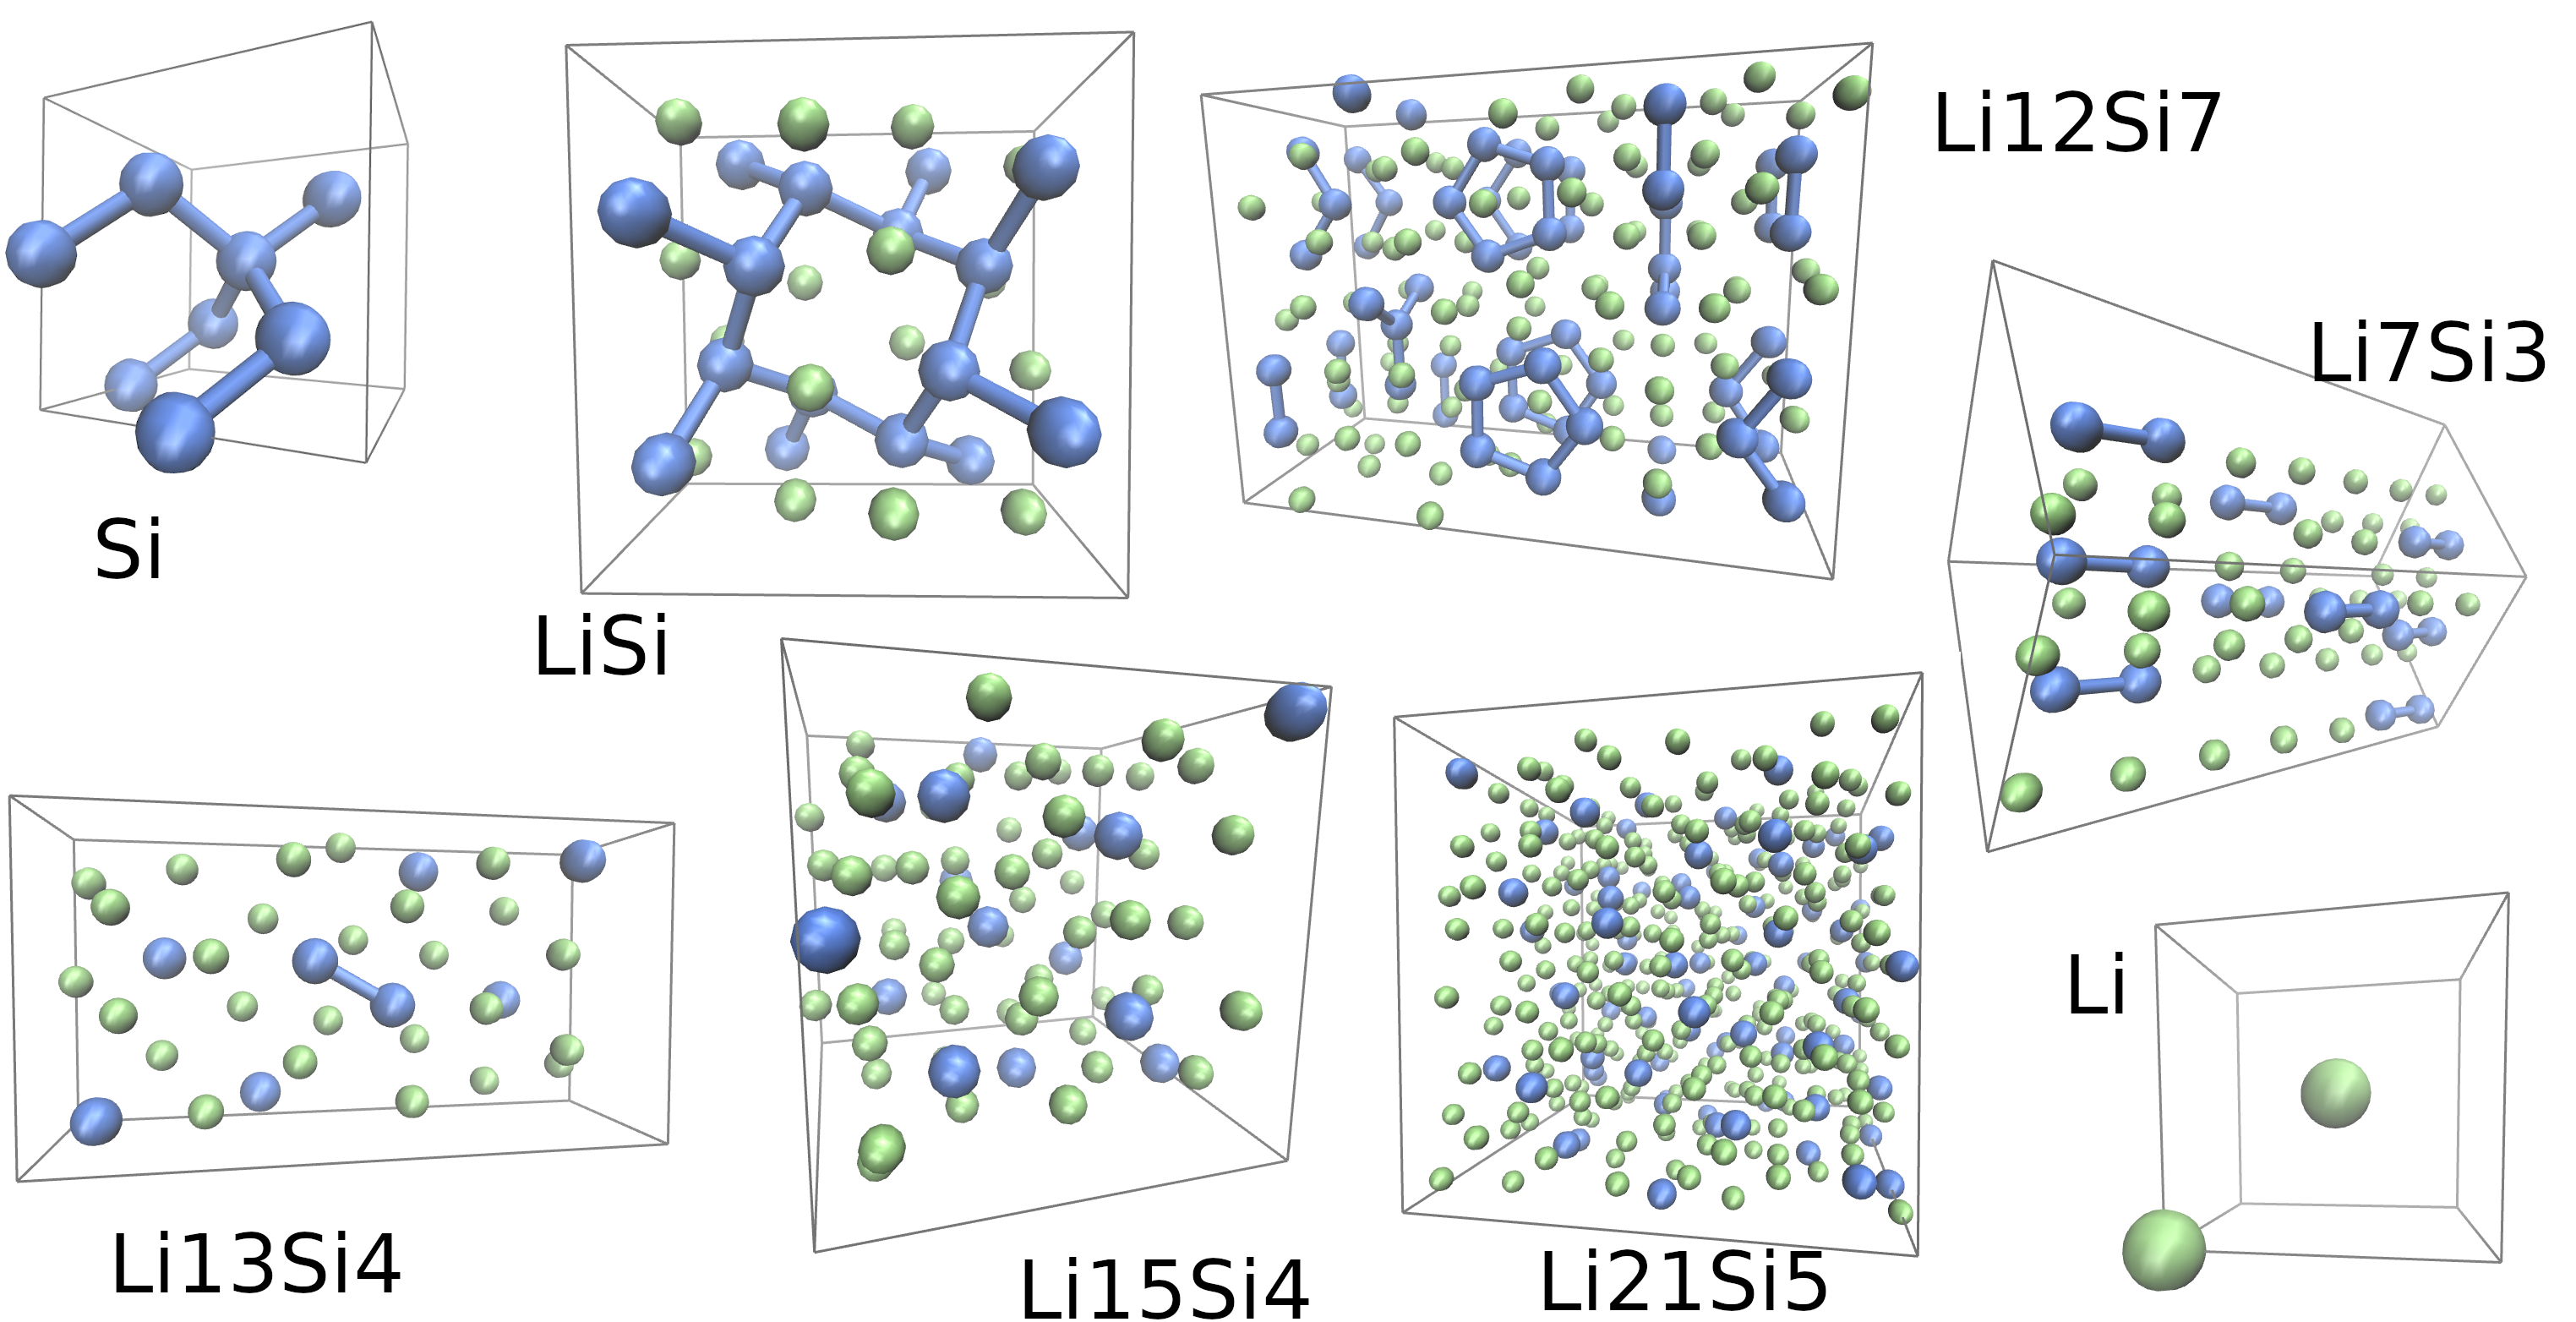
\includegraphics[width=\textwidth]{Silicio/caracterizacion/config/cristalinas.png}
    \caption{Estructuras cristalinas de Li-Si. Las estructuras no están a escala 
    entre sí. Los átomos de Si se muestran en azul y los de Li en verde, mientras
    que la celda periódica en gris. Los enlaces de Si-Si están graficados si la 
    distancia entre dos de estos átomos es menor a 3.0 \AA.}
    \label{fig:cristalinas}
\end{figure}

\subsection{Protocolo de delitiación}

Para obtener configuraciones iniciales para valores de $x$ distintos a los de las 
cristalinas se siguió un protocolo de delitiación, en el cual se selecciona la 
estructura cristalina más cercana con un valor de $x$ superior al deseado,
se le extrae un átomo de Li de manera aleatoria y se realiza una dinámica en el 
ensamble NPT durante 2 ps para relajar el volumen. Para estas simulaciones se 
utilizó el termostato de Nosé-Hoover ~\cite{nose1984a, nose1984b, hoover1985} a
300.0 K, un barostato a 0.0 atm y un paso temporal de 1 fs utilizando el
software \path{LAMMPS} ~\cite{lammps1, lammps2}. La extracción del átomo de Li y
la simulación en el ensamble NPT fueron repetidas hasta alcanzar una concentración
deseada. Por último, para algunas concentraciones en particular, se seleccionó la
estructura con la menor presión absoluta como estado inicial para la exploración 
acelerada de mínimos locales que se introduce en la siguiente sección.


% Copyright (c) 2024, Francisco Fernandez
% License: CC BY-SA 4.0
%   https://github.com/fernandezfran/thesis/blob/main/LICENSE
\subsection{Exploración acelerada de mínimos locales}\label{s:aelm}

Las simulaciones de MD tienen un gran poder predictivo para el estudio de 
procesos presentes en las baterías de litio, sin embargo, las escalas de tiempo
están limitadas a unos pocos ns o $\mu$s. El número de operaciones que se 
necesita para alcanzar las escalas de tiempo de la operación de una batería 
experimental son prohibitivos, incluso considerando el uso de potenciales 
semi-empíricos como el ReaxFF en supercomputadoras. Como consecuencia de esto,
la MD usual no es suficiente para una exploración del espacio de las fases y las
estructuras de Li-Si observadas van a estar cercanas a las configuraciones 
iniciales mientras que en el sistema real probablemente pueden aparecer otras
configuraciones. Un método simple y poderoso para acelerar la exploración de 
mínimos locales en sistemas moleculares es el templado simulado 
\cite{kirkpatrick1983}, en el cual básicamente se busca mejorar la exploración
del espacio de las fases en simulaciones de MD utilizando temperaturas altas y
luego reduciéndola progresivamente hasta encontrar un mínimo de energía a 
temperatura ambiente. El templado simulado múltiple (MSA, de sus siglas en inglés 
\textit{Multiple simluated annealing}) utiliza esta idea en distintas copias del 
sistema y fue utilizado para explorar y encontrar distintas estructuras mínimas 
relevantes cercanas al equilibrio \cite{hao2015}.

La presente técnica de simulación, exploración acelerada de mínimos locales (AELM,
de sus siglas en inglés \textit{accelerated exploration of local minima}), es 
similar a la MSA pero en vez de calentar y enfriar lentamente el sistema, se 
utiliza un sesgo en la función de energía potencial para sobrepasar las barreras
de energía y luego se realiza una minimización local, con algún minimizador local 
como gradientes conjugados o LBFGS, para encontrar el mínimo. Este método permite 
obtener muchas estructuras con energías mínimas relevantes, que son de interés a 
la hora de estudiar electrodos de Li-Si muy ciclados.

Las aleaciones de Li-Si presentan interacciones fuertes entre los átomos que las
conforman, especialmente en el enlace Si-Si donde la energía de enlace es del
orden de $\approx$2 eV \cite{wypych2018handbook}. Se espera que las barreras de 
energía potencial sean de ese orden de magnitud, por lo cual un 
muestreo de una MD a temperatura ambiente parece no ser viable. Para explorar 
ampliamente las distintas configuraciones del sistema, $\mathbf{r}$, se 
transforma la superficie de energía potencial (PES, de sus siglas en inglés 
\textit{potencial energy surface}), $V(\mathbf{r})$, usando un potencial sesgado
\begin{equation}\label{eq:bias}
    V_b(\mathbf{r}) = V(\mathbf{r}) + (\alpha - 1) V(\mathbf{r}) = \alpha V(\mathbf{r}),
\end{equation}
donde $\alpha$ es el factor de compresión. El principal efecto de la ecuación 
\ref{eq:bias} es reducir las barreras de la PES, por lo cual el tiempo de
residencia en estados metaestables es menor que en el sistema sin sesgar y la 
exploración de configuraciones de sistemas diferentes es más eficiente y 
alcanzada en un tiempo de simulación razonable. El término 
$(\alpha - 1) V(\mathbf{r})$ es usualmente referido como la 
\say{función de sesgo}.

La adición de esta función de sesgo a la PES constituye la base del método de 
hiper-dinámica (HD), desarrollado por Voter \cite{voter1997HD,voter1997method} 
para acelerar la exploración de un sistema sin perder su comportamiento dinámico a tiempos largos. En una 
simulación típica de HD, para recuperar el promedio de alguna propiedad, las 
configuraciones muestreadas son repesadas por un factor $w$ que involucra una función
exponencial y depende del sesgo aplicado. Debido a que este sistema involucra 
cambios grandes en las energías de interacción, comparado con la energía térmica
$k_BT$, lo que implica que la función exponencial en $w$ toma valores muy grandes,
esto provoca que el procedimiento numérico sea inestable y la recuperación de 
la propiedad de interés, como la energía potencial, no sea posible. Ya que este
capítulo se centra en un estudio estructural de los sistemas, podemos ignorar
el cálculo del tiempo real evolucionado en la simulación. Además, como el 
funcionamiento de las baterías luego se da a temperatura ambiente, es de esperar
que una vez que se alcance un mínimo local, el sistema explore configuraciones
cercanas a este. Por este motivo se aplica el método de gradientes conjugados (CG)
a cada una de las configuraciones de la HD y de esa forma se muestrea la 
multiplicidad de estructuras.

Este método de exploración introducido en esta tesis se asemeja al templado
simulado, aunque el objetivo es explorar muchas estructuras diferentes en vez de 
encontrar el mínimo global. El templado simulado fue utilizado anteriormente
con este mismo objetivo, Hao \textit{et al.} utilizó la técnica MSA para obtener
distintas estructuras de mínima energía de péptidos \cite{hao2015}. En este 
método AELM se usa HD en vez de temperaturas altas para favorecer la exploración,
y se realizan múltiples minimizaciones por CG en vez de simular un enfriado. 


\section{Resultados}

\section{Introducción}


\subsection{Comportamiento electroquímico}

\subsubsection{Cambio de volumen fraccionario}

El cambio de volumen fraccionario puede definirse utilizando una normalización 
relativa al número de átomos de Si en la estructura de acuerdo a
\begin{equation}\label{eq:fvc}
    \text{fvc} = \frac{N_{\text{Si}}}{V_{\text{Si}}} \left( \frac{V_{\text{Si},x}}{N_{\text{Si},x}} - \frac{V_{\text{Si}}}{N_{\text{Si}}} \right),
\end{equation}
donde $V_{\text{Si}}$ y $N_{\text{Si}}$ son el volumen y el número de átomos de 
Si en la celda unidad de c-Si, $V_{\text{Si},x}$ y $N_{\text{Si},x}$ son el 
volumen y el número de átomos de Si
en la celda de simulación para el valor correspondiente de $x$. En la Figura
\ref{fig:fvc} se muestran los valores calculados a partir de la ecuación 
\ref{eq:fvc} para las distintas estructuras de Li$_x$Si estudiadas. En la misma 
se comparan los valores obtenidos con datos experimentales de AFM (\textit{atomic 
force microscopy}, sus siglas en inglés) medidos por Beaulieu \textit{et al.} 
~\cite{beaulieu2003} y con predicciones de DFT con un cambio volumétrico fijo 
utilizado por Chevrier y Dahn ~\cite{chevrier2009}. Los mismos muestran que el
potencial ReaxFF proporciona una tendencia correcta, tanto cualitativa como 
cuantitativamente.
\begin{figure}[th]
    \centering
    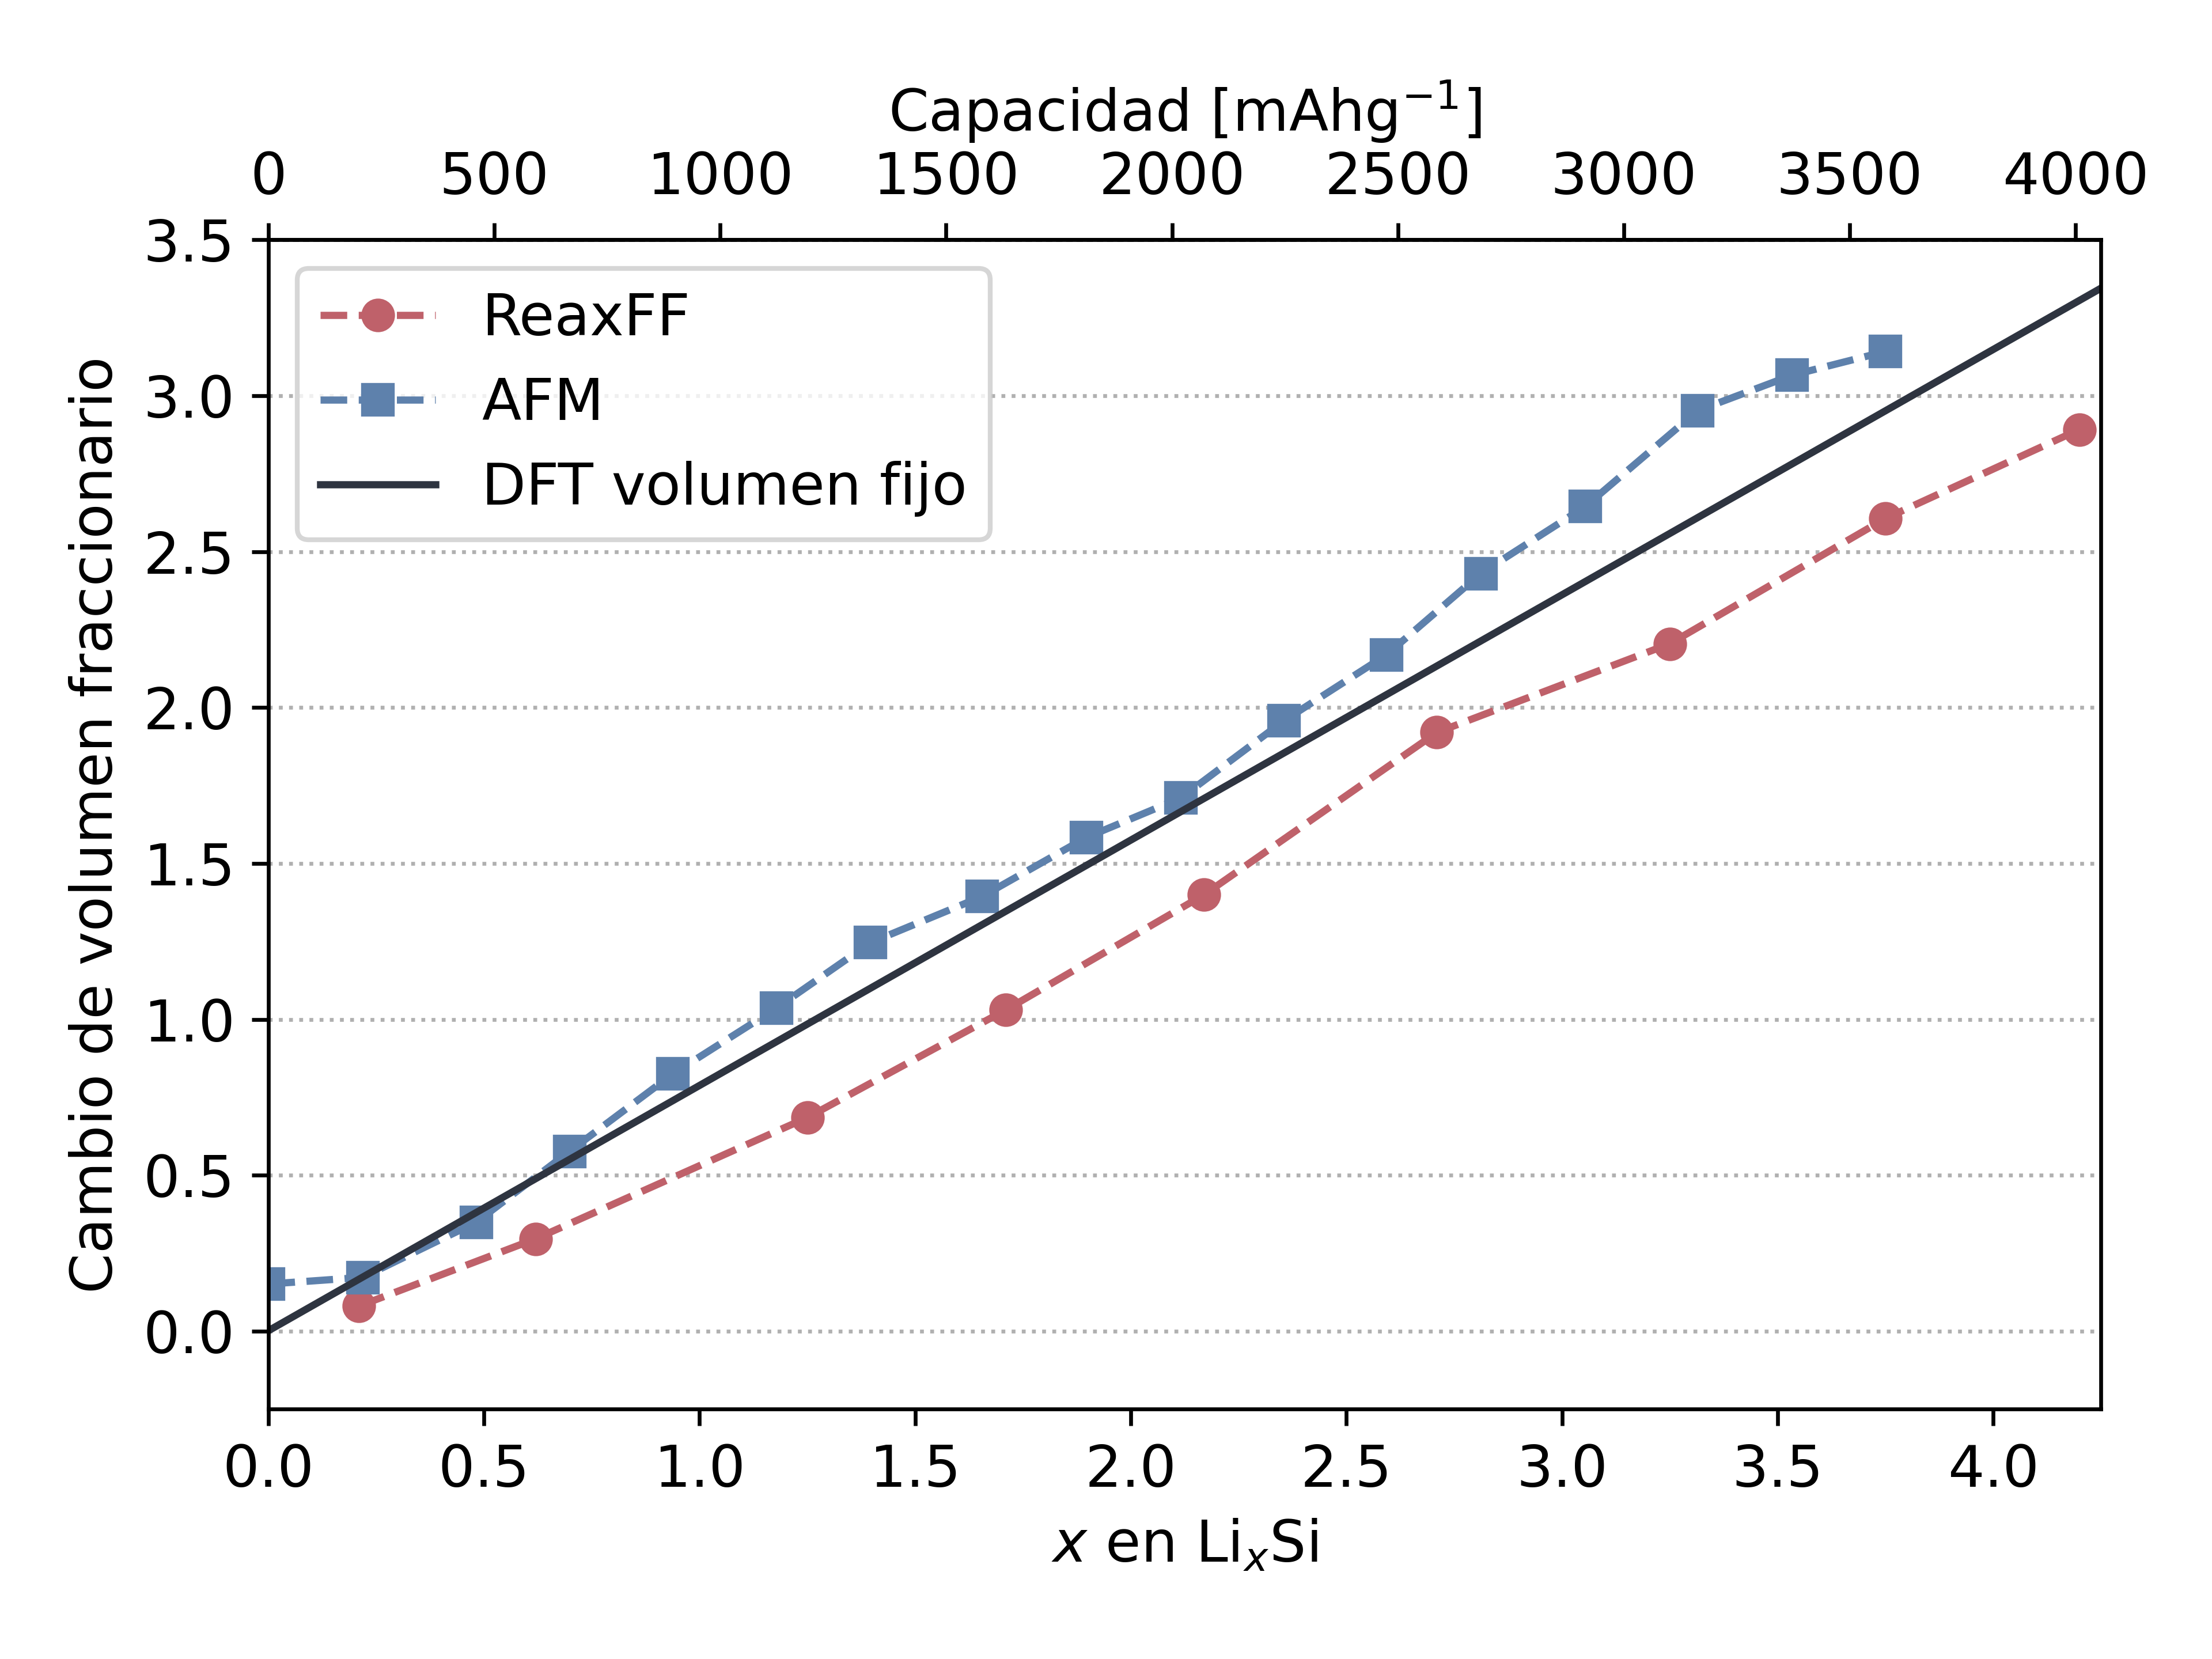
\includegraphics[width=0.8\textwidth]{Silicio/caracterizacion/resultados/electroquimica/fvc.png}
    \caption{Cambio de volumen fraccionario en función de la composición de la 
    aleación. Los valores experimentales de AFM se muestran con cuadrados azules, 
    la línea recta se corresponde con cálculos de DFT y los círculos rojos son 
    resultados de este trabajo.}
    \label{fig:fvc}
\end{figure}

\subsubsection{Voltaje}

\begin{table}[h]
    \centering
    \caption{Energías de formación obtenidas a través de la ecuación \ref{eq:fe}}
    \setlength\extrarowheight{2pt}\stackon{%
    \begin{tabular}{c c}
        \toprule
        \textbf{x en Li$_x$Si} & 
        \textbf{Energía de formación [eV]} \\ 
        \midrule
        0.21  &  0.503 $\pm$ 0.003 \\
        0.62  &  0.121 $\pm$ 0.007 \\
        1.25  & -0.12 $\pm$ 0.01 \\
        1.71  & -0.236 $\pm$ 0.007 \\
        2.17  & -0.355 $\pm$ 0.008 \\
        2.71  & -0.410 $\pm$ 0.007 \\
        3.25  & -0.52 $\pm$ 0.01 \\
        3.75  & -0.62 $\pm$ 0.01 \\
        4.20  & -0.699 $\pm$ 0.008 \\
        \bottomrule
    \end{tabular}
    }{}
    \label{t:fe}
\end{table}
Las energías obtenidas pueden ser utilizadas para evaluar el funcionamiento del 
modelo para predecir propiedades electroquímicas, como fue sugerido por Chevrier
y Dahn ~\cite{chevrier2009}. Primero, se define la energía de formación de las 
distintas estructuras amorfas como
\begin{equation}\label{eq:fe}
    E_f(x) = E_{\text{Li}_x\text{Si}} - (x E_{\text{Li}} + E_{\text{Si}}),
\end{equation}
donde $E_{\text{Li}_x\text{Si}}$ es la energía de la aleación Li$_x$Si por átomo 
de Si, $E_{\text{Li}}$ y $E_{\text{Si}}$ son las energías cohesivas de Li y Si
en sus fases cristalinas. Usando
la ecuación \ref{eq:fe} como aproximación a la energía de formación de Gibbs, el 
potencial \textit{versus} Li metálico de Li$_x$Si puede obtenerse a partir de
\begin{equation}\label{eq:voltaje}
    V(x) = - \frac{dE_f(x)}{dx},
\end{equation}
donde $V$ es el potencial. Los datos obtenidos así pueden compararse con valores
experimentales y computacionales previos. Las energías de formación calculadas
a partir de la ecuación \ref{eq:fe} se muestran en la Tabla \ref{t:fe}. 
Si se realiza un \textit{spline} a estos valores, mostrados en el recuadro de la
Figura \ref{fig:voltaje}, se obtienen los valores de $V(x)$ a partir de la ecuación
\ref{eq:voltaje}, que se grafican en función de la composición en la Figura 
\ref{fig:voltaje} con una línea roja. Para comparar, se incluye en la misma Figura
las curvas experimentales medidas para la litiación y la delitiación de silicio
amorfo ~\cite{hatchard2004} y la curva teórica de cálculos de primeros principios 
~\cite{chevrier2009}. Se puede afirmar que los resultados obtenidos con el ReaxFF 
son satisfactorios.
\begin{figure}[th]
    \centering
    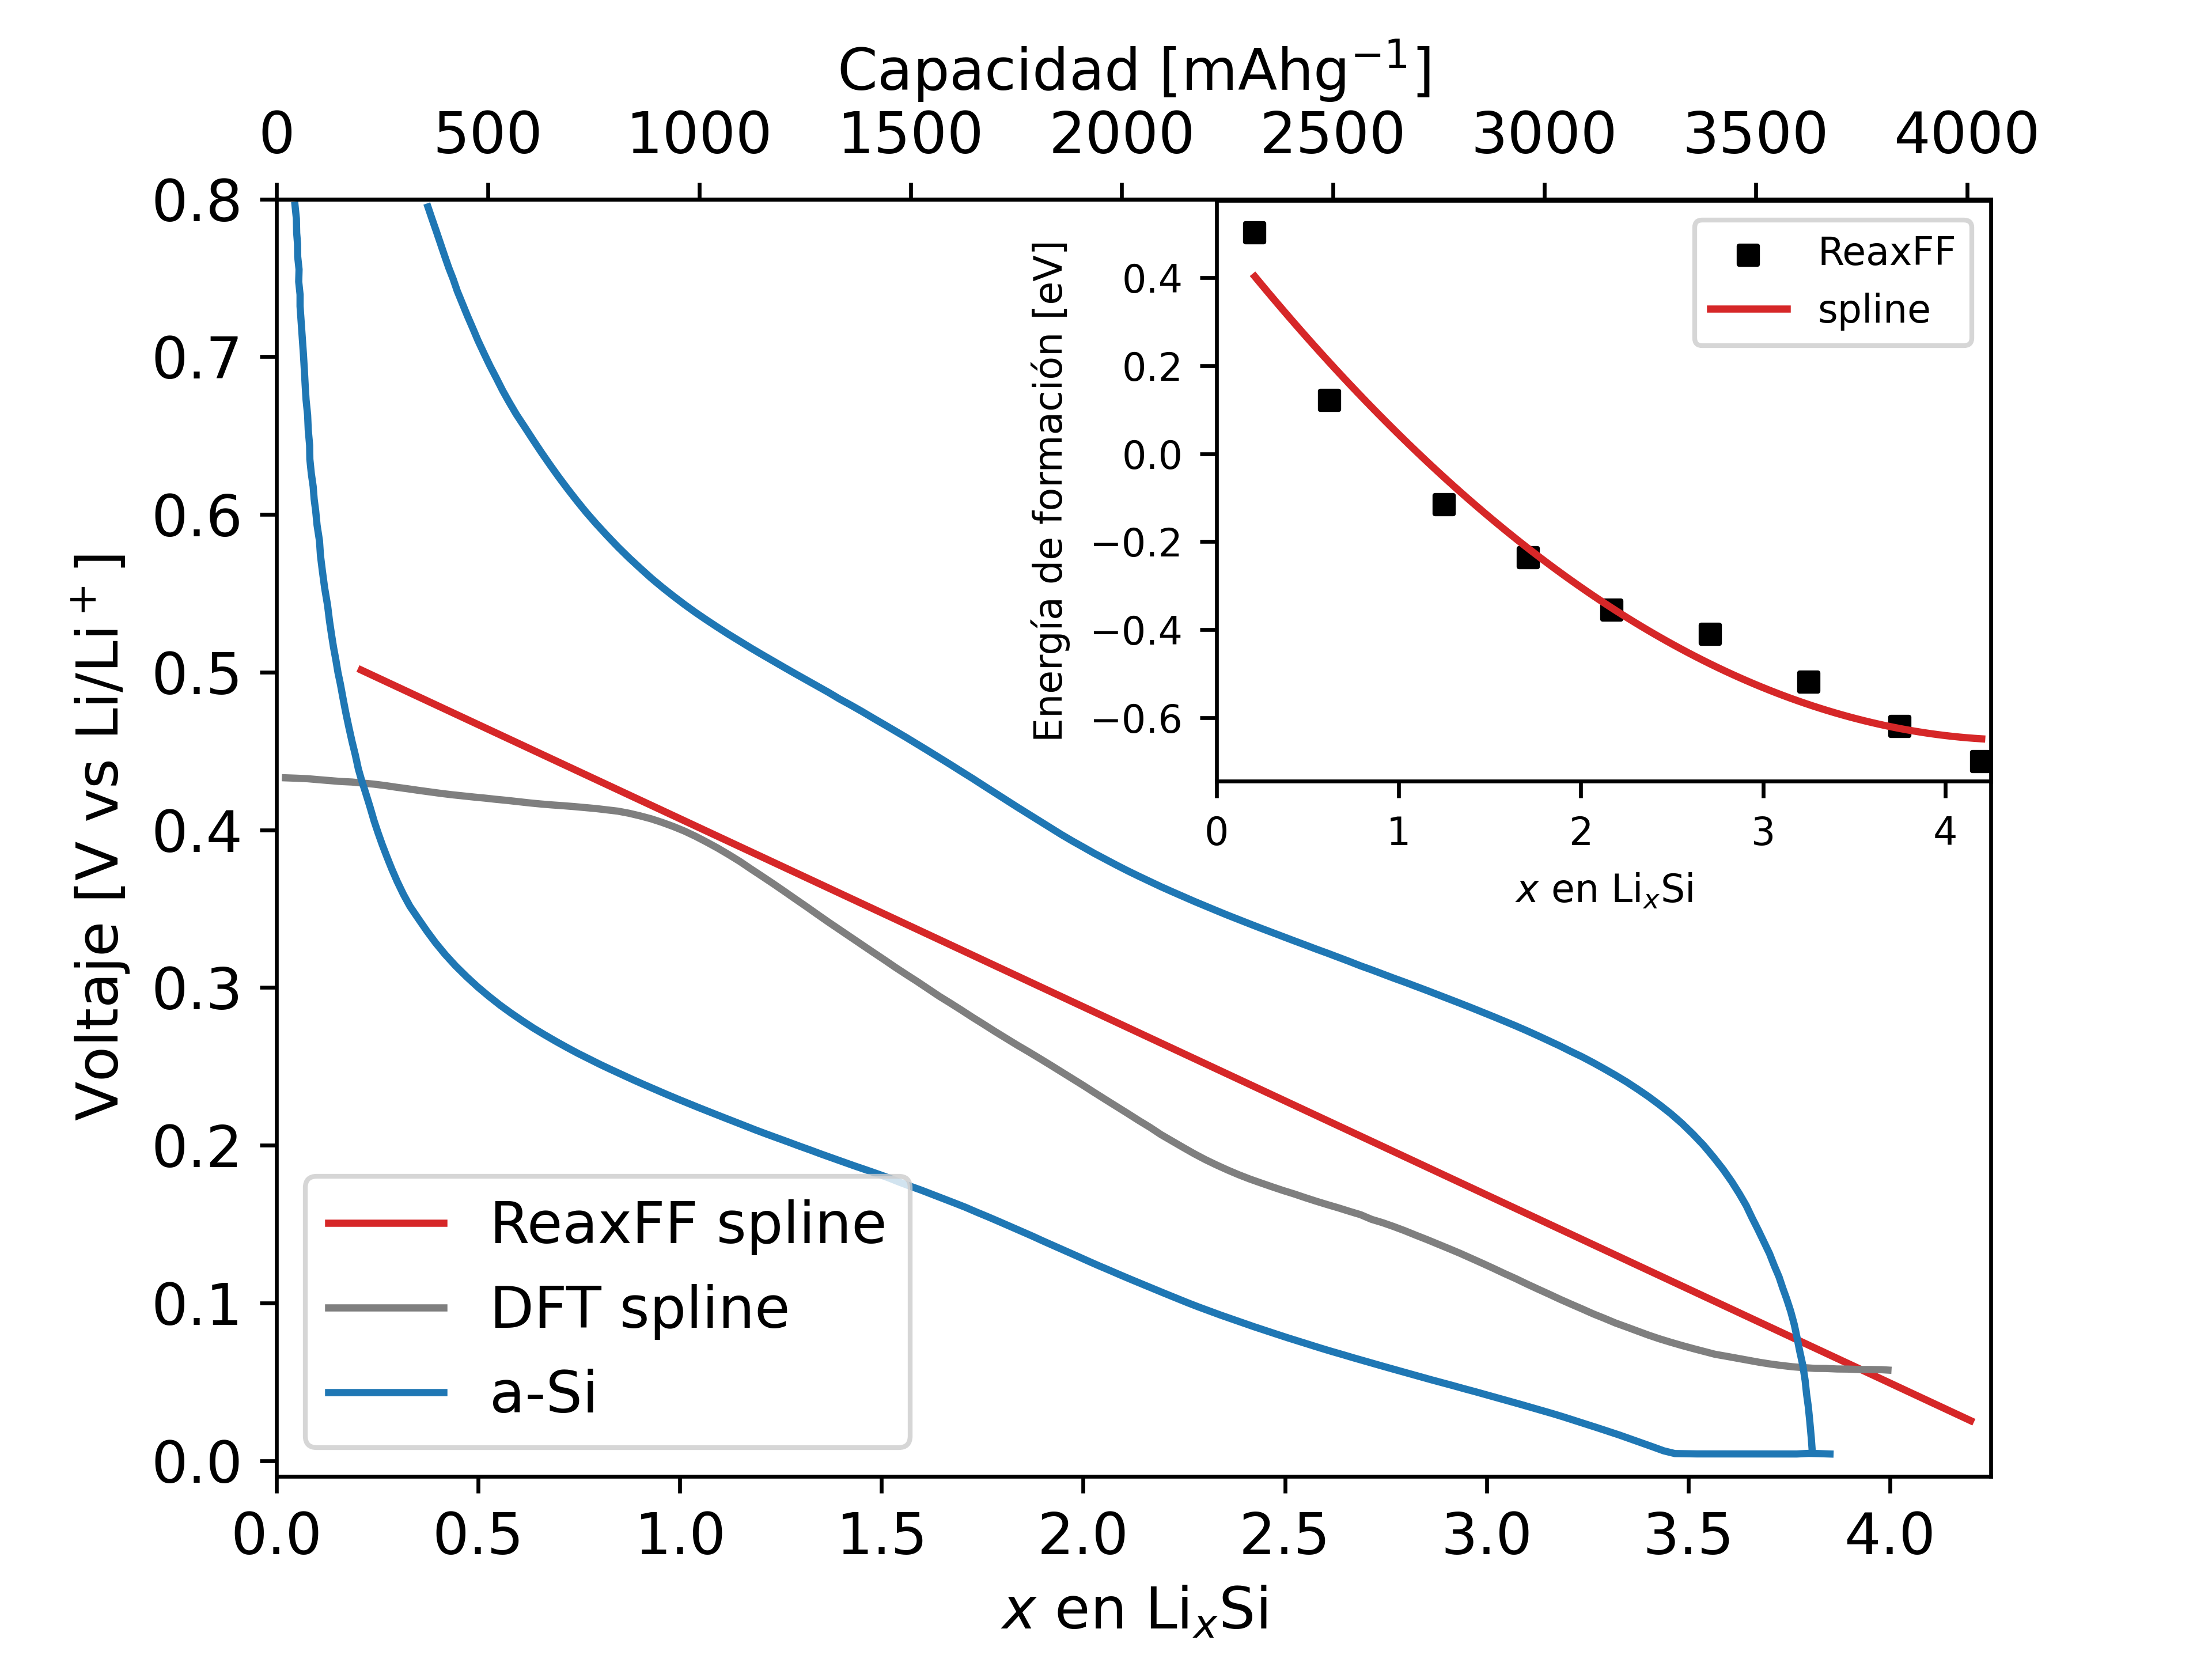
\includegraphics[width=0.8\textwidth]{Silicio/caracterizacion/resultados/electroquimica/voltaje.png}
    \caption{Curvas potencial-concentración para la litiación de ánodos de Si.
    La línea negra corresponde a cálculos de DFT, las líneas azules a 
    curvas medidas experimentalmente en la litiación de Si amorfo y la línea 
    roja es la derivada del \textit{spline} ajustado a los datos de la energía 
    de formación obtenidos con el ReaxFF, presentados en el recuadro.}
    \label{fig:voltaje}
\end{figure}


\subsection{Amorfización del silicio mediante un templado simulado y análisis de la función de distribución radial (RDF)}\label{s:rdfb}

Por último, las mayores discrepancias entre las energías de formación calculadas con DFTB
con respecto a DFT se corresponden a estructuras de silicio amorfo, por lo cual,
se realizó una evaluación extra para este caso. En la Figura \ref{fig:rdfb} se 
muestran las RDFs Si-Si (ver ecuación \ref{eq:rdf}) obtenidas por un templado simulado para cada una de las
parametrizaciones. Además, se compara con el potencial previo de ReaxFF 
\cite{fan2013} y con una determinación experimental \cite{laaziri1999}. Para 
obtener las estructuras amorfas se comenzó con una celda de c-Si con 64 átomos 
a la cual se le realizó un templado simulado en el ensamble $NVT$ utilizando el 
termostato de Nosé-Hoover. El mismo consistió en una etapa inicial de 
calentamiento lineal desde temperatura ambiente hasta 3000 K durante 100 ps, luego una
termalización a dicha temperatura por 600 ps y, por último, un enfriamiento 
exponencial de 600 ps hasta llegar a temperatura ambiente. Para todas las etapas
se utilizó un paso temporal de 1 fs. Para el cómputo de las RDFs que se muestran
en la Figura \ref{fig:rdfb} se equilibró la estructura alcanzada a temperatura 
ambiente durante 100 ps. Puede destacarse que los resultados del conjunto B de parámetros muestran
una concordancia excelente con los datos experimentales de la referencia 
\cite{laaziri1999}, lo que convierte a esta parametrización en la más adecuada
para simulaciones futuras. Los archivos de dichos parámetros están disponibles
en un repositorio público \cite{dftb_lisi}.
\begin{figure}[h!]
    \centering
    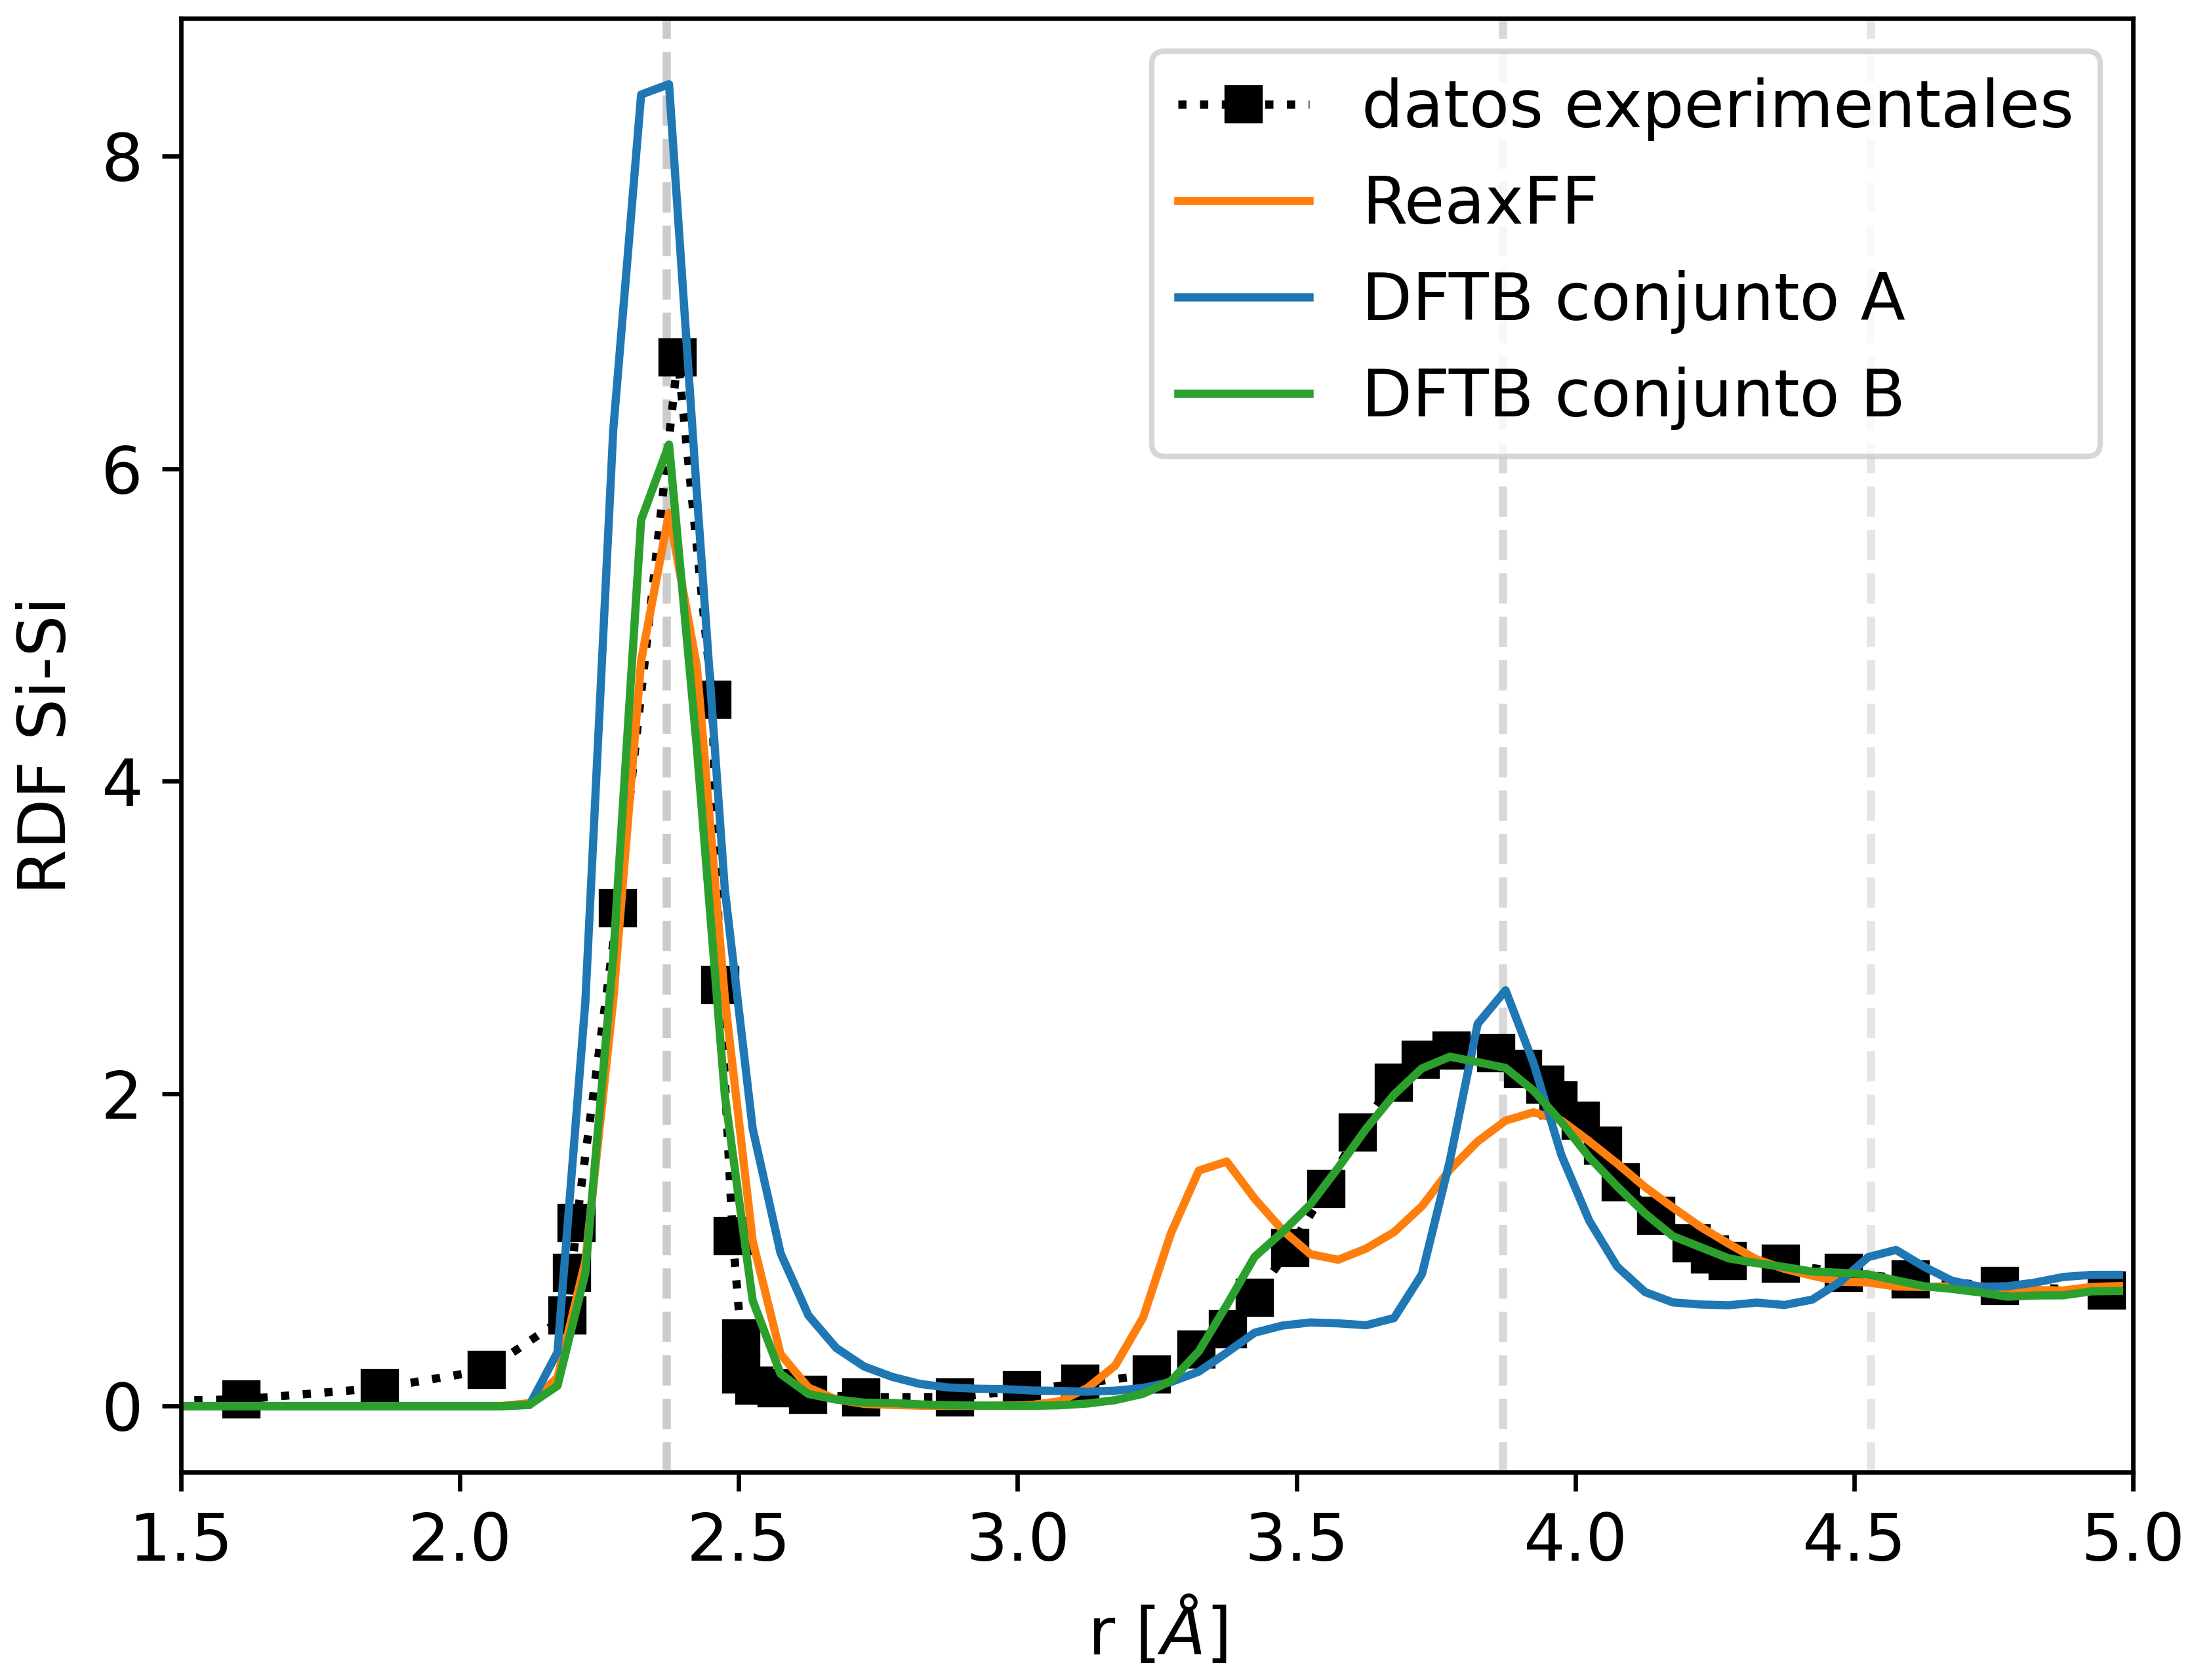
\includegraphics[width=.7\textwidth]{Silicio/modelo/resultados/rdf/rdf.png}
    \caption{Función de distribución radial (RDF) de silicio amorfo para los
    conjuntos A y B de parametrizaciones. Los resultados se comparan con 
    mediciones de la referencia \cite{laaziri1999} y con los resultados obtenidos
    utilizando el ReaxFF \cite{fan2013}. Las líneas grises discontinuas verticales
    muestran dónde estarían los picos del silicio cristalino a 0 K. Se encuentra 
    una concordancia excelente entre el experimento y la parametrización del 
    conjunto B.}
    \label{fig:rdfb}
\end{figure}


% Copyright (c) 2024, Francisco Fernandez
% License: CC BY-SA 4.0
%   https://github.com/fernandezfran/thesis/blob/main/LICENSE
\subsection{Número de coordinación}

De la misma manera que se utilizaron las distribuciones radiales parciales, se pueden
obtener los números de coordinación para un dado tipo de átomo utilizando la ecuación
\ref{eq:cn} definida en la sección \ref{ss:cn} con la $g(r)$ correspondiente. Debido
a que en los materiales amorfos la primera y la segunda esfera de coordinación pueden 
llegar a estar superpuestas, el límite superior de integración no está definido 
unívocamente para todas las concentraciones consideradas \cite{lamparter1995}.
El número de coordinación promedio para átomos de Si vecinos de otros átomos 
de Si se calculó utilizando un radio de 
corte de 3 \AA. Lo mismo se realizó para Li-Li definiendo un radio de corte de 
4 \AA. Para el caso de Si-Li se utilizó el criterio de considerar como radio de 
corte el valor $r$ para el cual la $g(r)$ presenta un mínimo entre los dos picos
a primeros y segundo vecinos. Los resultados se muestran en la Figura 
\ref{fig:cn}a.
\begin{figure}[h!]
    \centering
    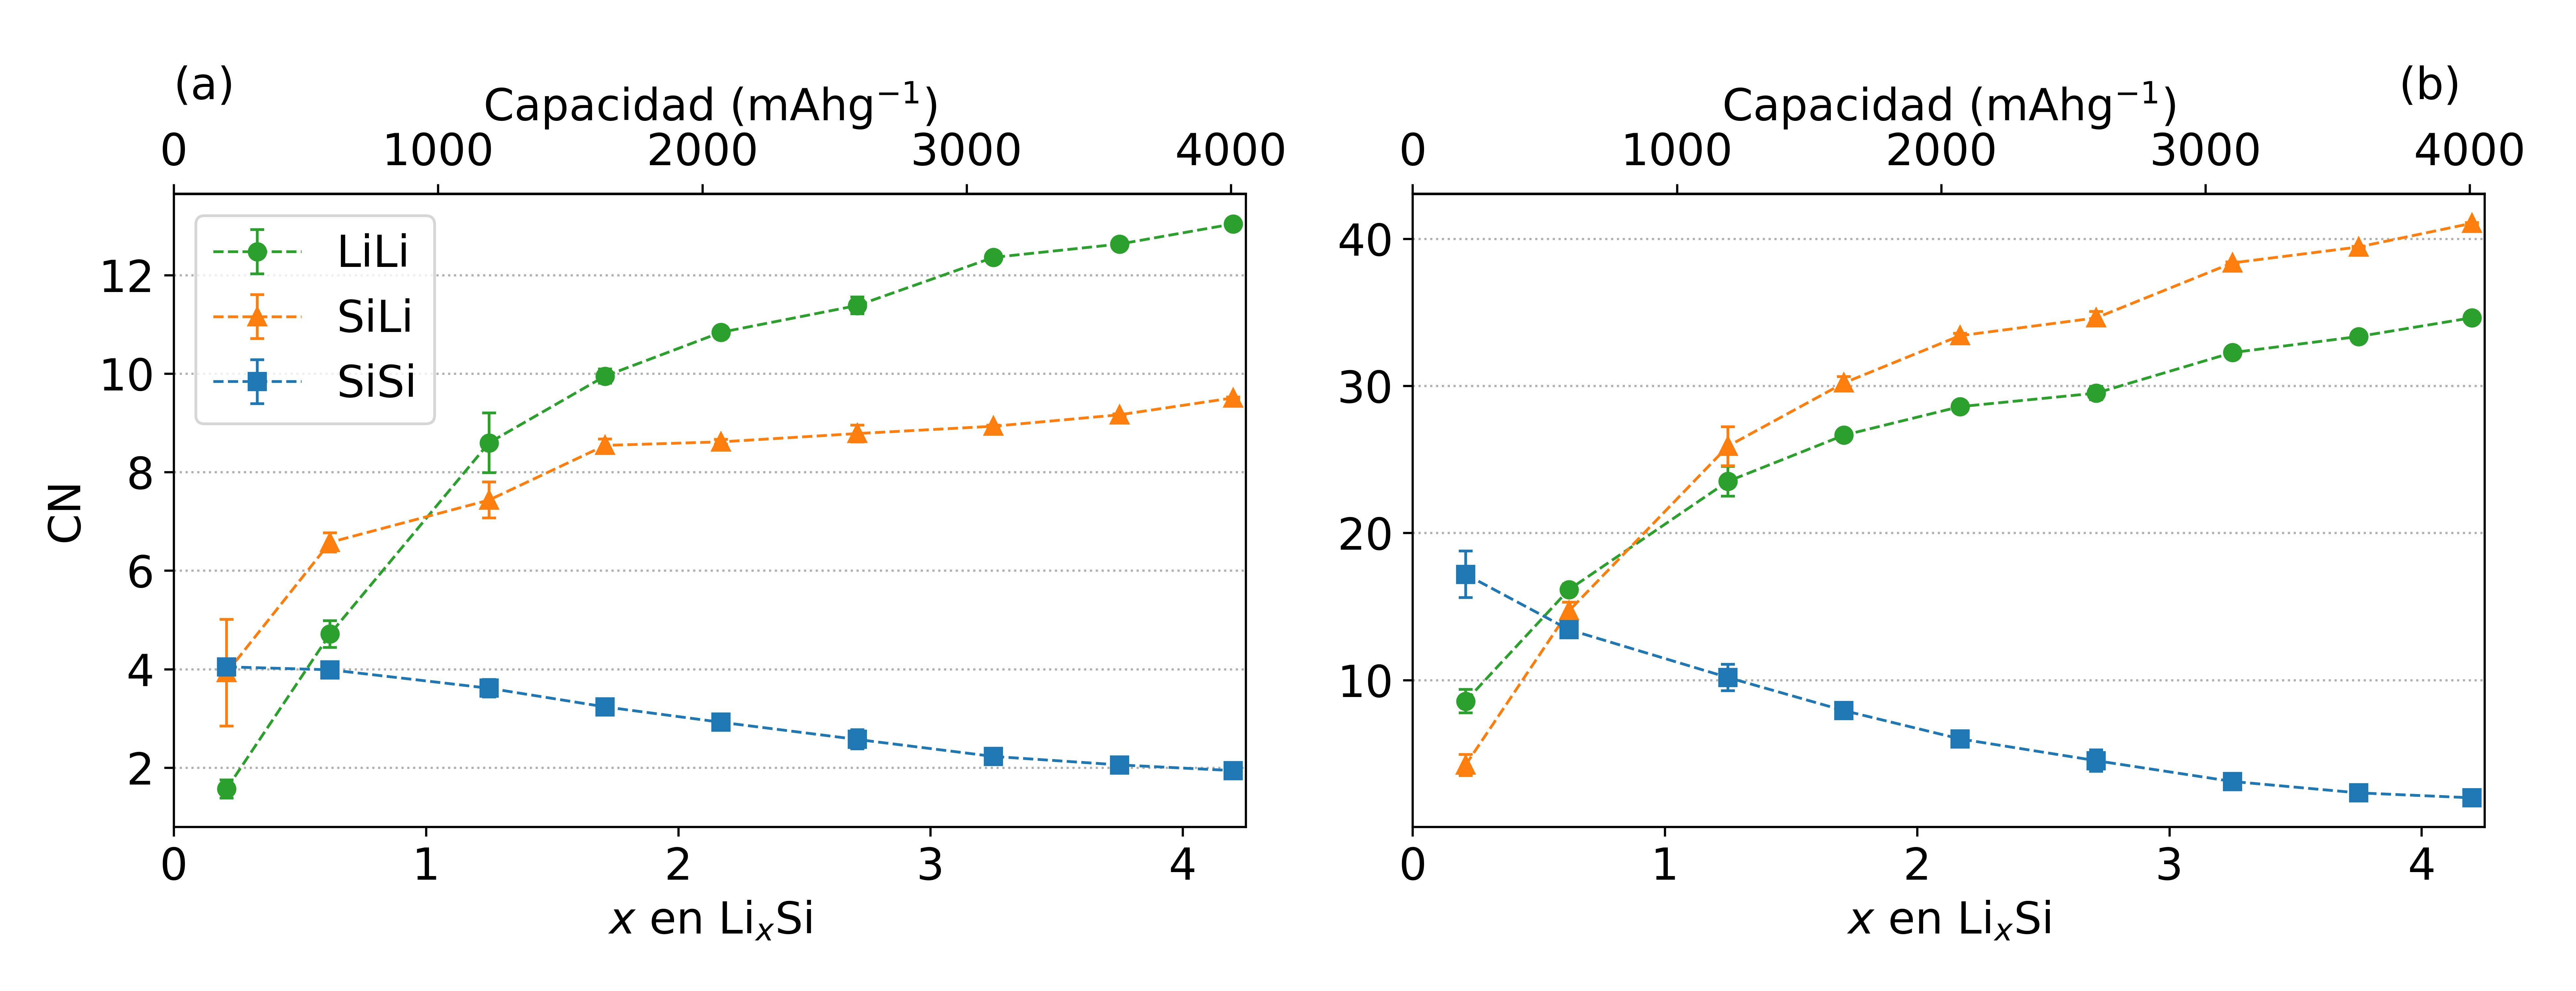
\includegraphics[width=\textwidth]{Silicio/caracterizacion/resultados/cn/cn.png}
    \caption{Número de coordinación en función de la concentración de litio para
    Li-Li, Si-Si y Si-Li. Como radios de corte se utilizaron las distancias 
    del pico de la RDF correspondiente. En los casos en que no se aprecia la barra
    de error, la misma es menor que el tamaño de los puntos. (a) Primero número 
    de coordinación. (b) Segundo número de coordinación.}
    \label{fig:cn}
\end{figure}

Para el caso del CN$_{\text{Si}-\text{Si}}$, se tiene que esta cantidad decrece de 4 a 2, a 
medida que la concentración de Li aumenta. Esto indica que a valores pequeños de 
$x$ la estructura de Si mantiene sus conexiones tetraédricas, mientras que para
valores grandes de $x$ el Si tiende a formar cadenas periódicas unidimensionales.
En la red de silicio amorfa, analizada con más detalle en la sección 
\ref{s:clusters}, se presenta una estructura 3d-periódica para valores bajos de 
$x$, donde el CN se encuentra alrededor de 4. Luego, se alcanza una estructura 1d-periódica 
para valores grandes de $x$, donde los enlaces Si-Si tienden a formar 
cadenas, que pueden verse para $x = 3.75$ donde se tiene CN = 2.05, por ejemplo.
El CN de Si-Li y Li-Li presenta valores pequeños para concentraciones 
bajas y aumenta monótonamente hasta alcanzar valores de 10 y 12, respectivamente, 
que se asemejan al valor de una estructura de empaquetamiento compacto.

Los resultados para el segundo número de coordinación se presentan en la Figura 
\ref{fig:cn}b. Estos resultados se obtuvieron considerando un cascarón con un 
radio de corte interno y otro externo, elegidos de manera tal que incluyan el 
segundo pico de la RDF. La elección de dichos valores varió dependiendo del tipo
de átomos que se consideraron. En todos ellos se tomó como radio de corte interno 
el radio de corte del primero número de coordinación. Luego, para el radio de 
corte externo se utilizaron valores de 5.0 \AA\ para Si-Si y 6.0 \AA\ para Li-Li
y Si-Li.

Para los valores de CN$_{\text{Si}-\text{Si}}$ se observa un aumento para concentraciones bajas
de Li, si se lo compara con el CN de primeros vecinos. Para valores mayores de $x$,
se puede ver cómo el valor de CN también tiende a 2, lo cual es coherente con la
formación de cadenas que se notó previamente. La tendencia cualitativa del segundo
CN para Li-Li y Si-Li es la misma que la observada en el primer CN, sólo que ahora
empieza en un valor cercano a 5 y tiende a 35 y 40, respectivamente. Este valor 
es mucho mayor que el que se tiene para los segundos vecinos en una estructura 
de empaquetamiento compacto, que es 6 para la estructura cristalina FCC. Incluso 
es mayor a la suma del segundo (6) y del tercer vecino (24) esperado para la red 
FCC.


% Copyright (c) 2024, Francisco Fernandez
% License: CC BY-SA 4.0
%   https://github.com/fernandezfran/thesis/blob/main/LICENSE
\subsection{Formación de conglomerados (clusters)}\label{s:clusters}

Analizando la formación de \change{conglomerados} (clusters) por medio del algoritmo DBSCAN 
\cite{ester1996}, en el cual puede definirse un radio de corte para el cual se 
deja de considerar que los átomos están enlazados entre sí (es decir, formando 
clusters), se encuentra que las estructuras amorfas de silicio no pueden ser 
clasificadas en diferentes tipos de clusters, las mismas reflejan más bien 
una red amorfa. Esto viene de interpretar los gráficos que se presentan en la 
Figura \ref{fig:clusters}. 
\begin{figure}[h!]
    \centering
    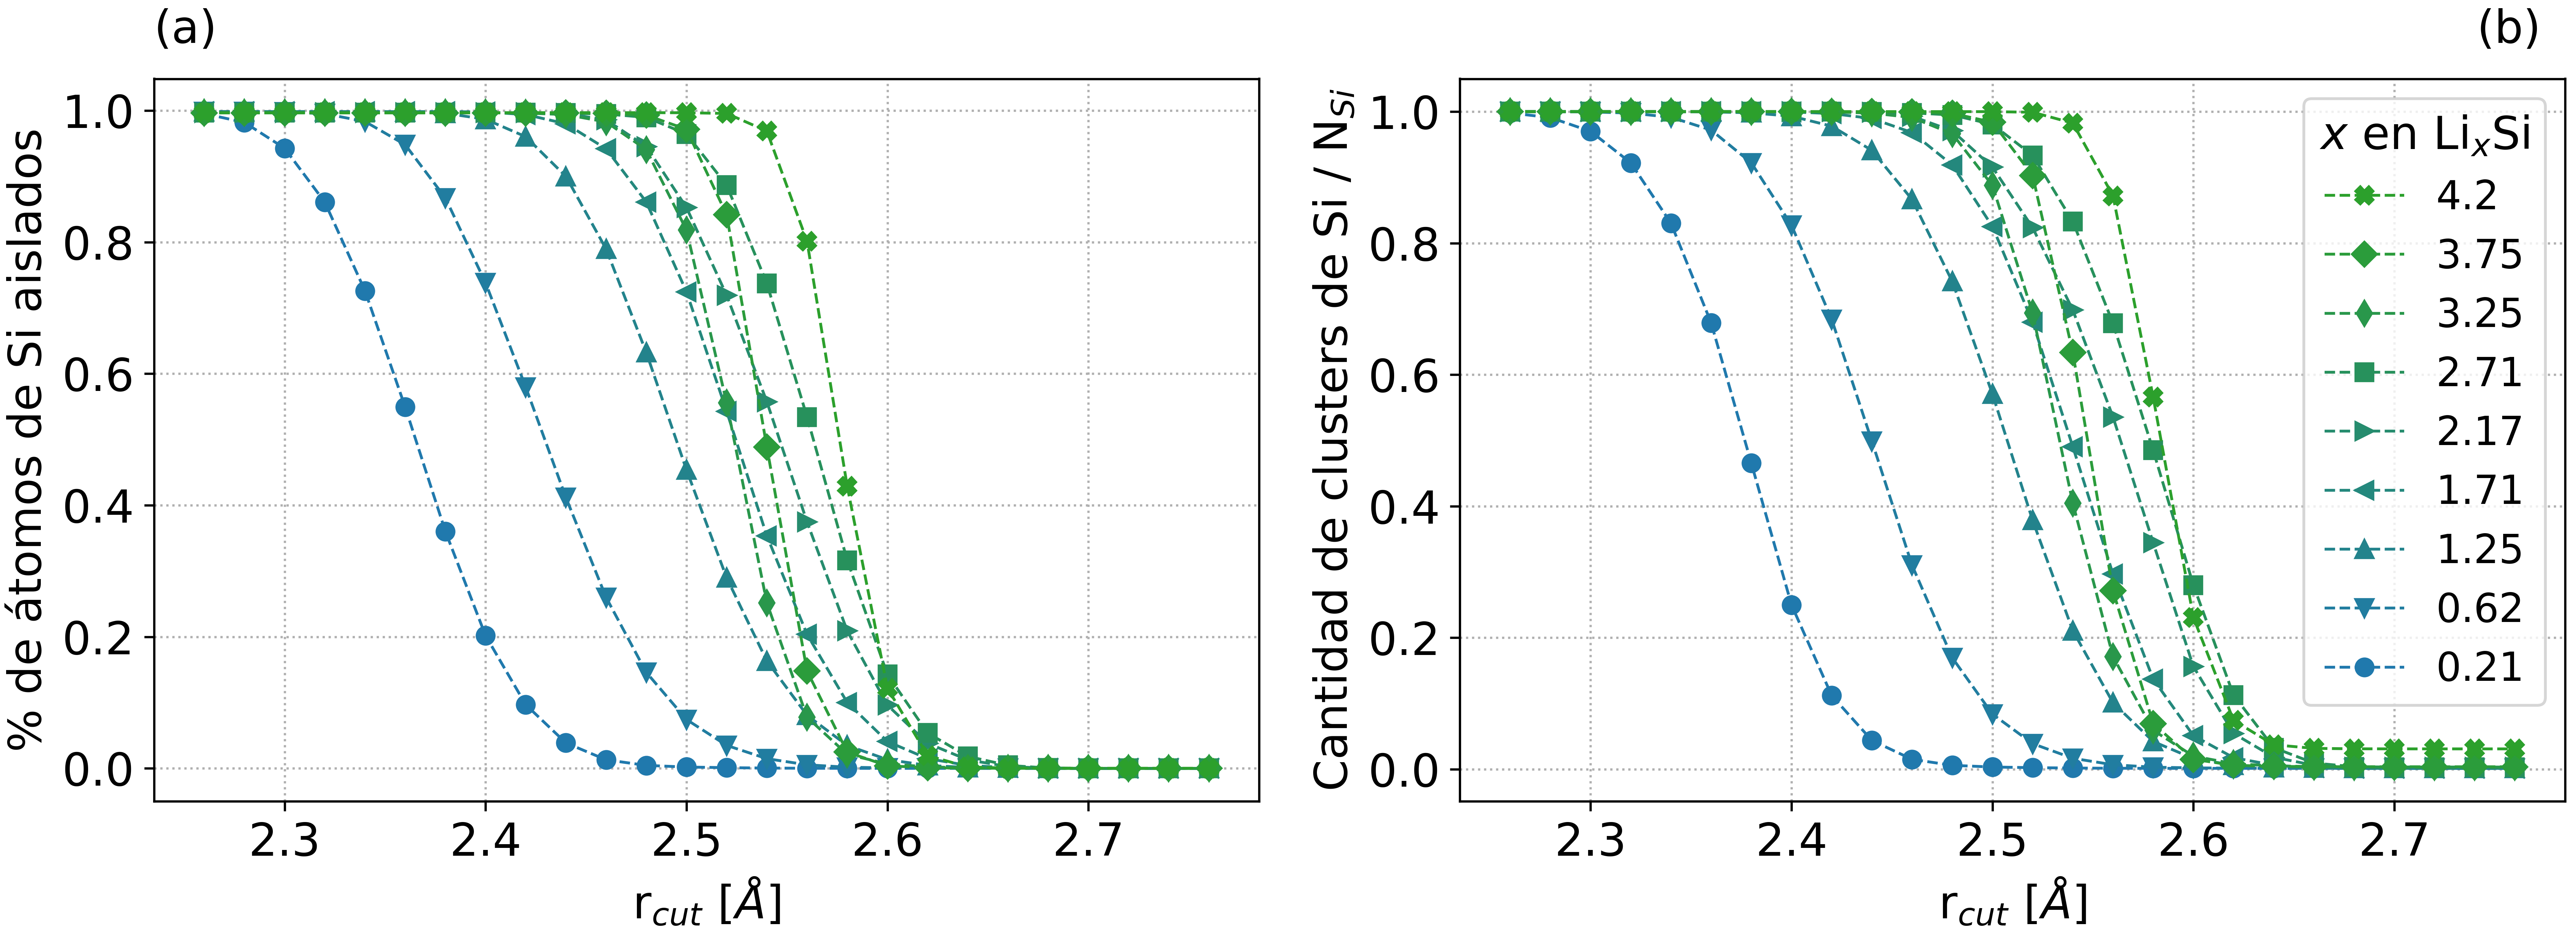
\includegraphics[width=\textwidth]{Silicio/caracterizacion/resultados/clusters/clusters.png}
    \caption{Formación de clusters indicando una red amorfa de silicio. (a) 
    Fracción de átomos de Si aislados en función de la elección del
    radio de corte. (b) Número de clusters de Si sobre el número total de átomos 
    de Si.}
    \label{fig:clusters}
\end{figure}

En particular, en la Figura \ref{fig:clusters}a se define la fracción 
de átomos de Si que están a una distancia mayor que $r_{cut}$ de otros átomos de 
Si. Cuando el radio de corte es mayor que la distancia a la cual termina el 
primer pico de la RDF$_{\text{Si}-\text{Si}}$, no se tienen átomos de Si que cumplan esta 
propiedad, es decir, no hay átomos de Si que se encuentren aislados en el sistema,
incluso a concentraciones altas de Li. Esto refleja que el a-Si se comporta como 
una red en la cual todos los átomos de silicio están interconectados entre sí, 
cosa que también se puede deducir de la Figura \ref{fig:clusters}b, en la cual 
se tiene que cuando el radio de corte es menor que el primer pico de la RDF$_{\text{Si}-\text{Si}}$ 
el número de clusters es igual al número de átomos de Si, pero que cuando este 
radio es más grande que la distancia a la cual termina el primer pico, hay un 
solo cluster.


\subsection{Interconexión de clusters}\label{s:interconexion}

Para determinar qué es lo que genera una estructura compleja en el segundo pico de la 
RDF$_{\text{Si}-\text{Li}}$, ver Figura \ref{fig:rdf}, se realizó un análisis similar al reportado por Ding \textit{et al.}
\cite{ding2015}. Estos autores analizaron la correlación en la distancia de a
pares de los segundos vecinos más cercanos en términos de las conexiones entre
clusters, definiendo un poliedro de coordinación alrededor del átomo central 
considerado para la RDF y sus segundos vecinos. El número de átomos compartidos
entre estos dos poliedros de coordinación enlazados fueron utilizados para 
establecer categorías y analizar sus contribuciones a la RDF. Estas categorías
dependen del hecho de que los poliedros comparten un vértice (1 átomo), una 
arista (2 átomos), una cara de los poliedros (3 átomos) o cuadriláteros 
distorsionados o tetraedros aplastados (4 átomos). De una forma similar al trabajo de Ding, se deconvolucionó el segundo pico de la RDF calculando la RDF parcial 
de distintas categorías, donde cada categoría se define por el número de átomos de
Li que interconectan un átomo de Si con su segundo vecino de Li. El comportamiento
detallado se presenta en la Figura \ref{fig:interconexiones}. Puede afirmarse a 
grandes rasgos que para concentraciones bajas de Li en las aleaciones, hay una 
predominancia de segundos vecinos de Li que tienen una o ninguna interconexión 
con los vecinos de Li de la primera esfera de coordinación Si-Li. Para $x > 1.0$
la contribución del segundo vecino de Li interconectado con dos o más átomos de 
Li de la primera esfera de coordinación Si-Li comienza a ser predominante y la
contribución de los átomos de Li sin conectarse empieza a decaer. Para $x > 3.0$,
la contribución del primer pico del segundo vecino de Li interconectado dos o
tres veces se vuelve relevante mientras que aparecen contribuciones de cuatro o
más interconexiones.
\begin{figure}[h!]
    \centering
    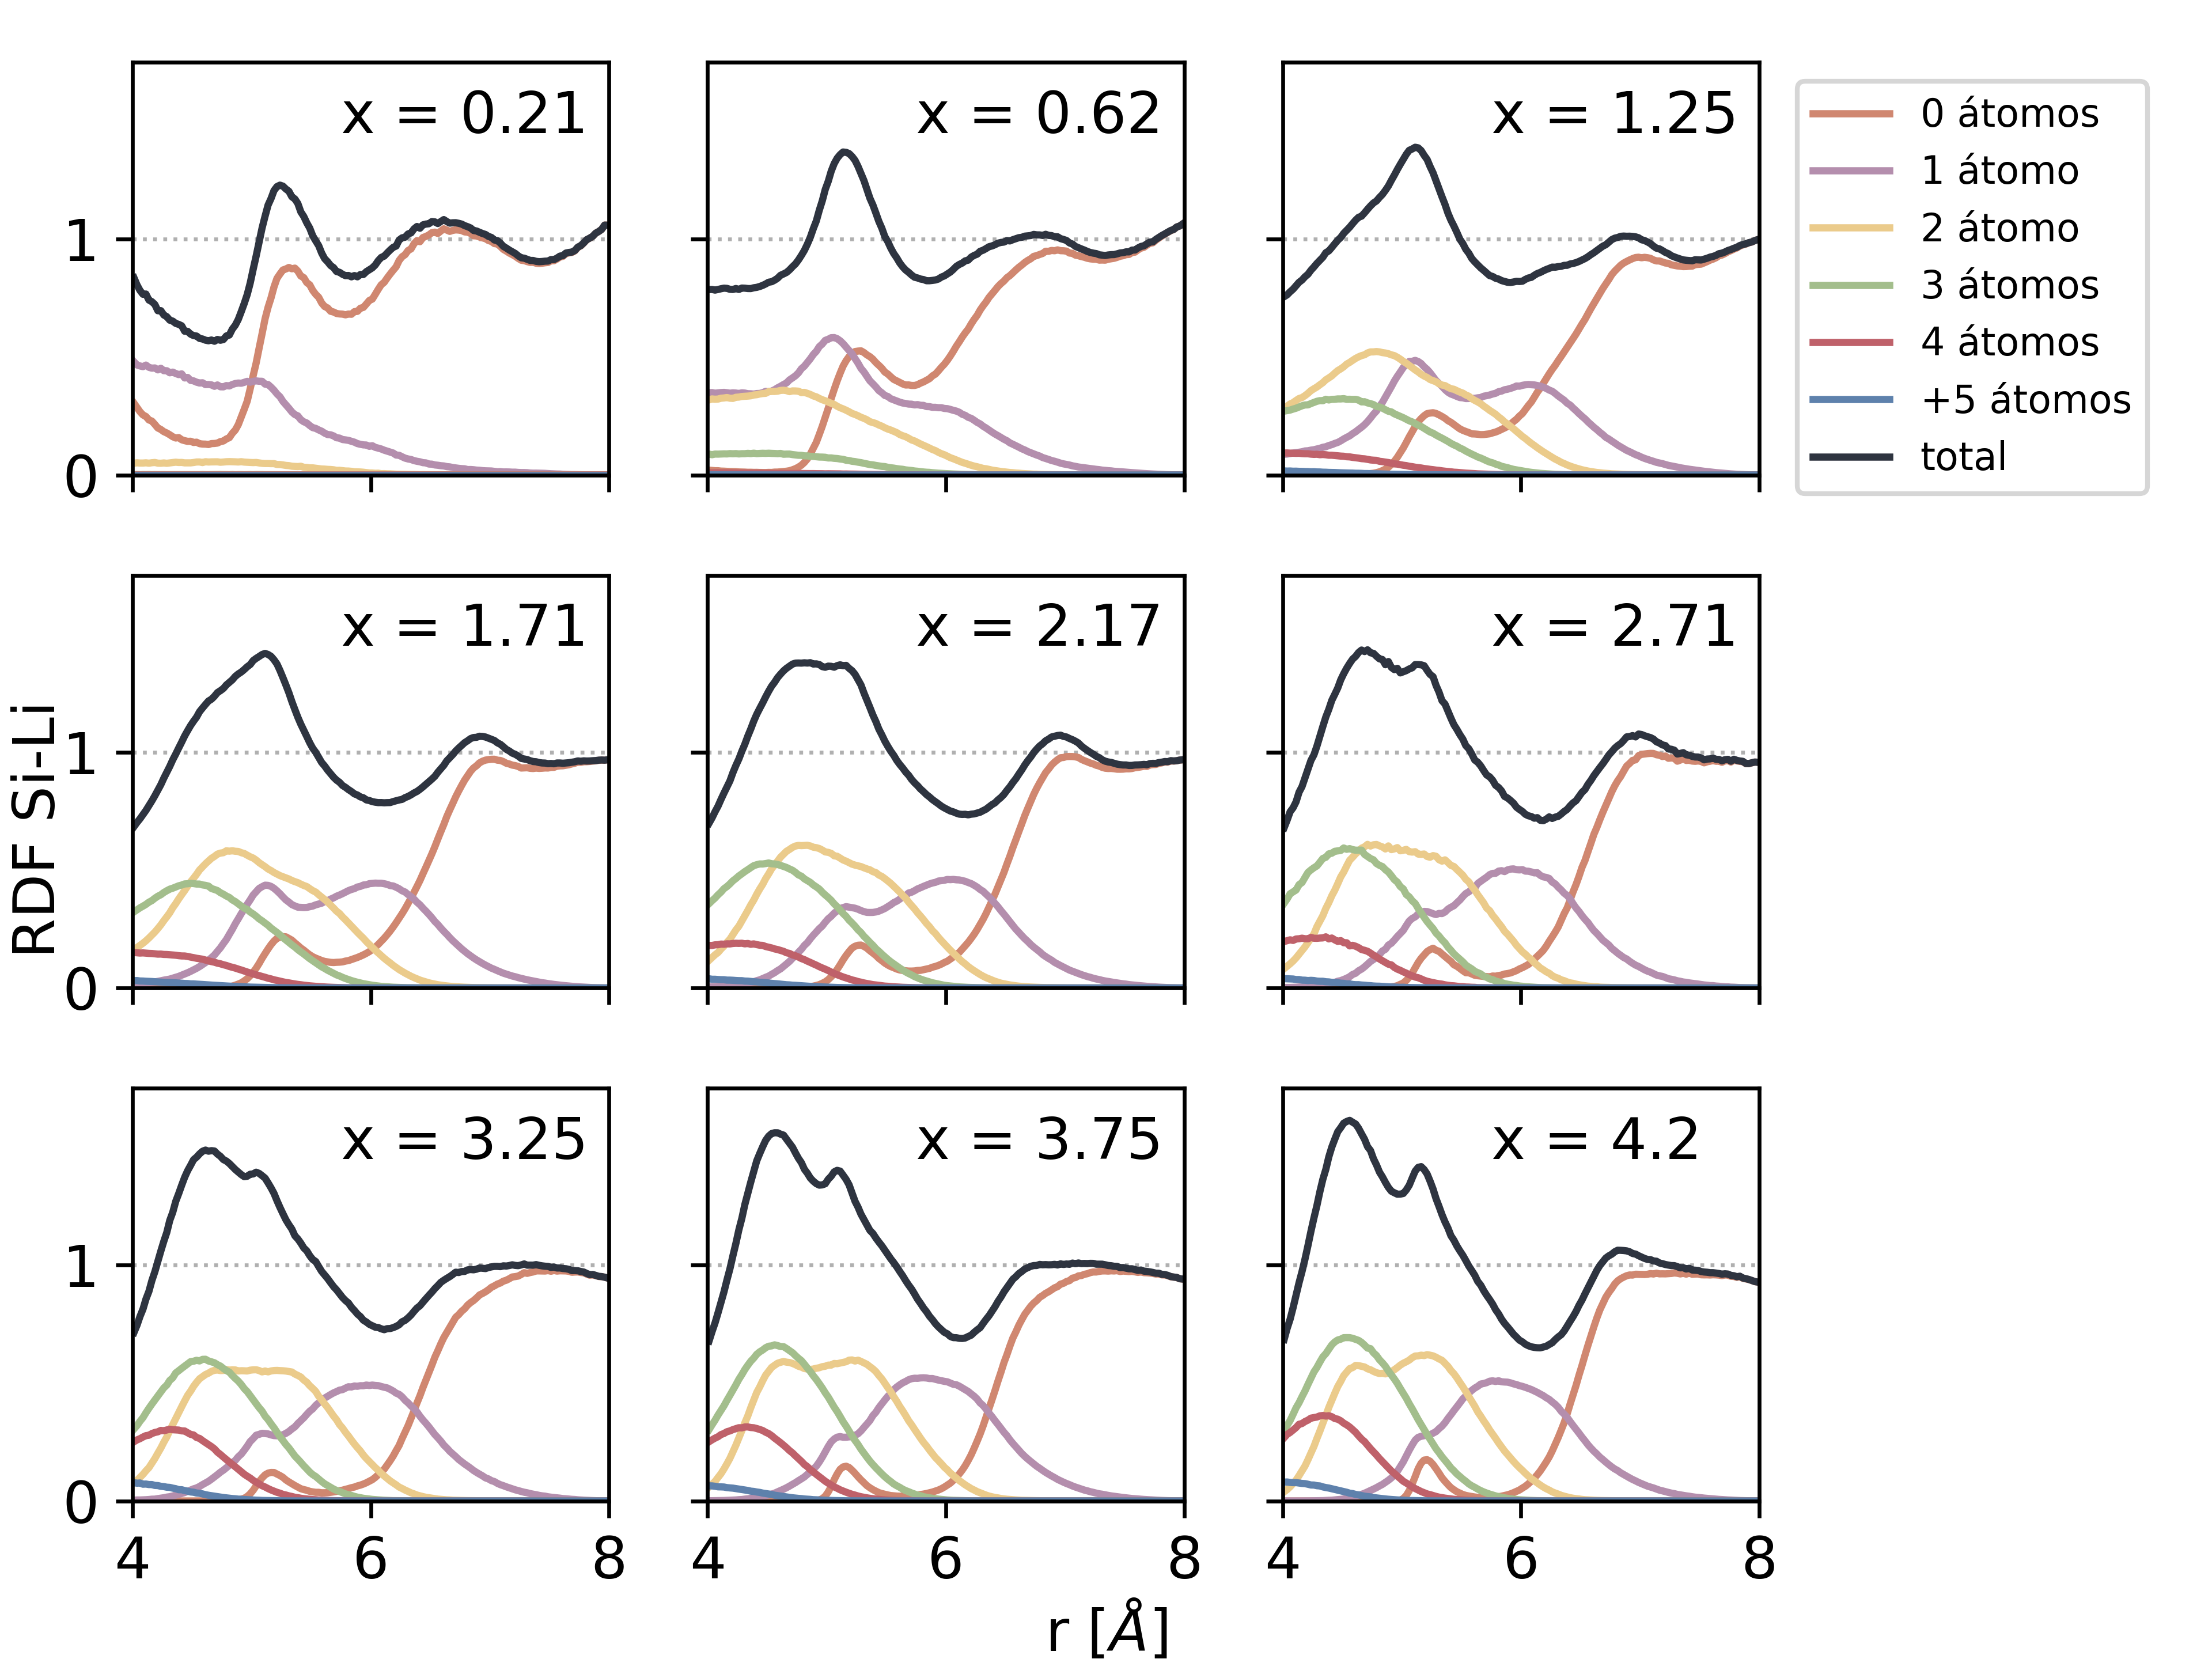
\includegraphics[width=\textwidth]{Silicio/caracterizacion/resultados/interconexion/interconexiones.png}
    \caption{Interconexiones de los segundos vecinos más cercanos de Li con un 
    átomo central de Si para cada valor de $x$ en Li$_x$Si considerado \cite{ding2015}. El número 
    de primeros vecinos más cercanos que conectan a los segundos vecinos más 
    cercanos con el átomo central de Si se indica en el recuadro de las figuras. 
    Además de la RDF$_{\text{Si}-\text{Li}}$ total, se grafica cada una de las contribuciones 
    de los diferentes tipos de interconexiones posibles.}
    \label{fig:interconexiones}
\end{figure}

Mientras que el comportamiento presentado en la Figura \ref{fig:interconexiones}
es más bien complejo, pueden establecerse tendencias generales que ayudan a 
entender mejor que es lo que sucede. Si se divide la RDF$_{\text{Si}-\text{Li}}$ en dos 
contribuciones de segundos vecinos, la primera de ellas, que se encuentra a una
distancia entre 4.0 \AA\ y 5.0 \AA, se puede atribuir a los átomos que tienen dos 
o más interconexiones de Li, mientras que la segunda de ellas, entre 5.0 \AA\ y
5.6 \AA, se corresponde con los átomos que tiene una o ninguna interconexión de 
Li. Utilizando esta clasificación, se muestra en la Figura 
\ref{fig:interconexiones-areas} la fracción del área que representa cada una de
estas categorías en función de la concentración de litio.
\begin{figure}[h!]
    \centering
    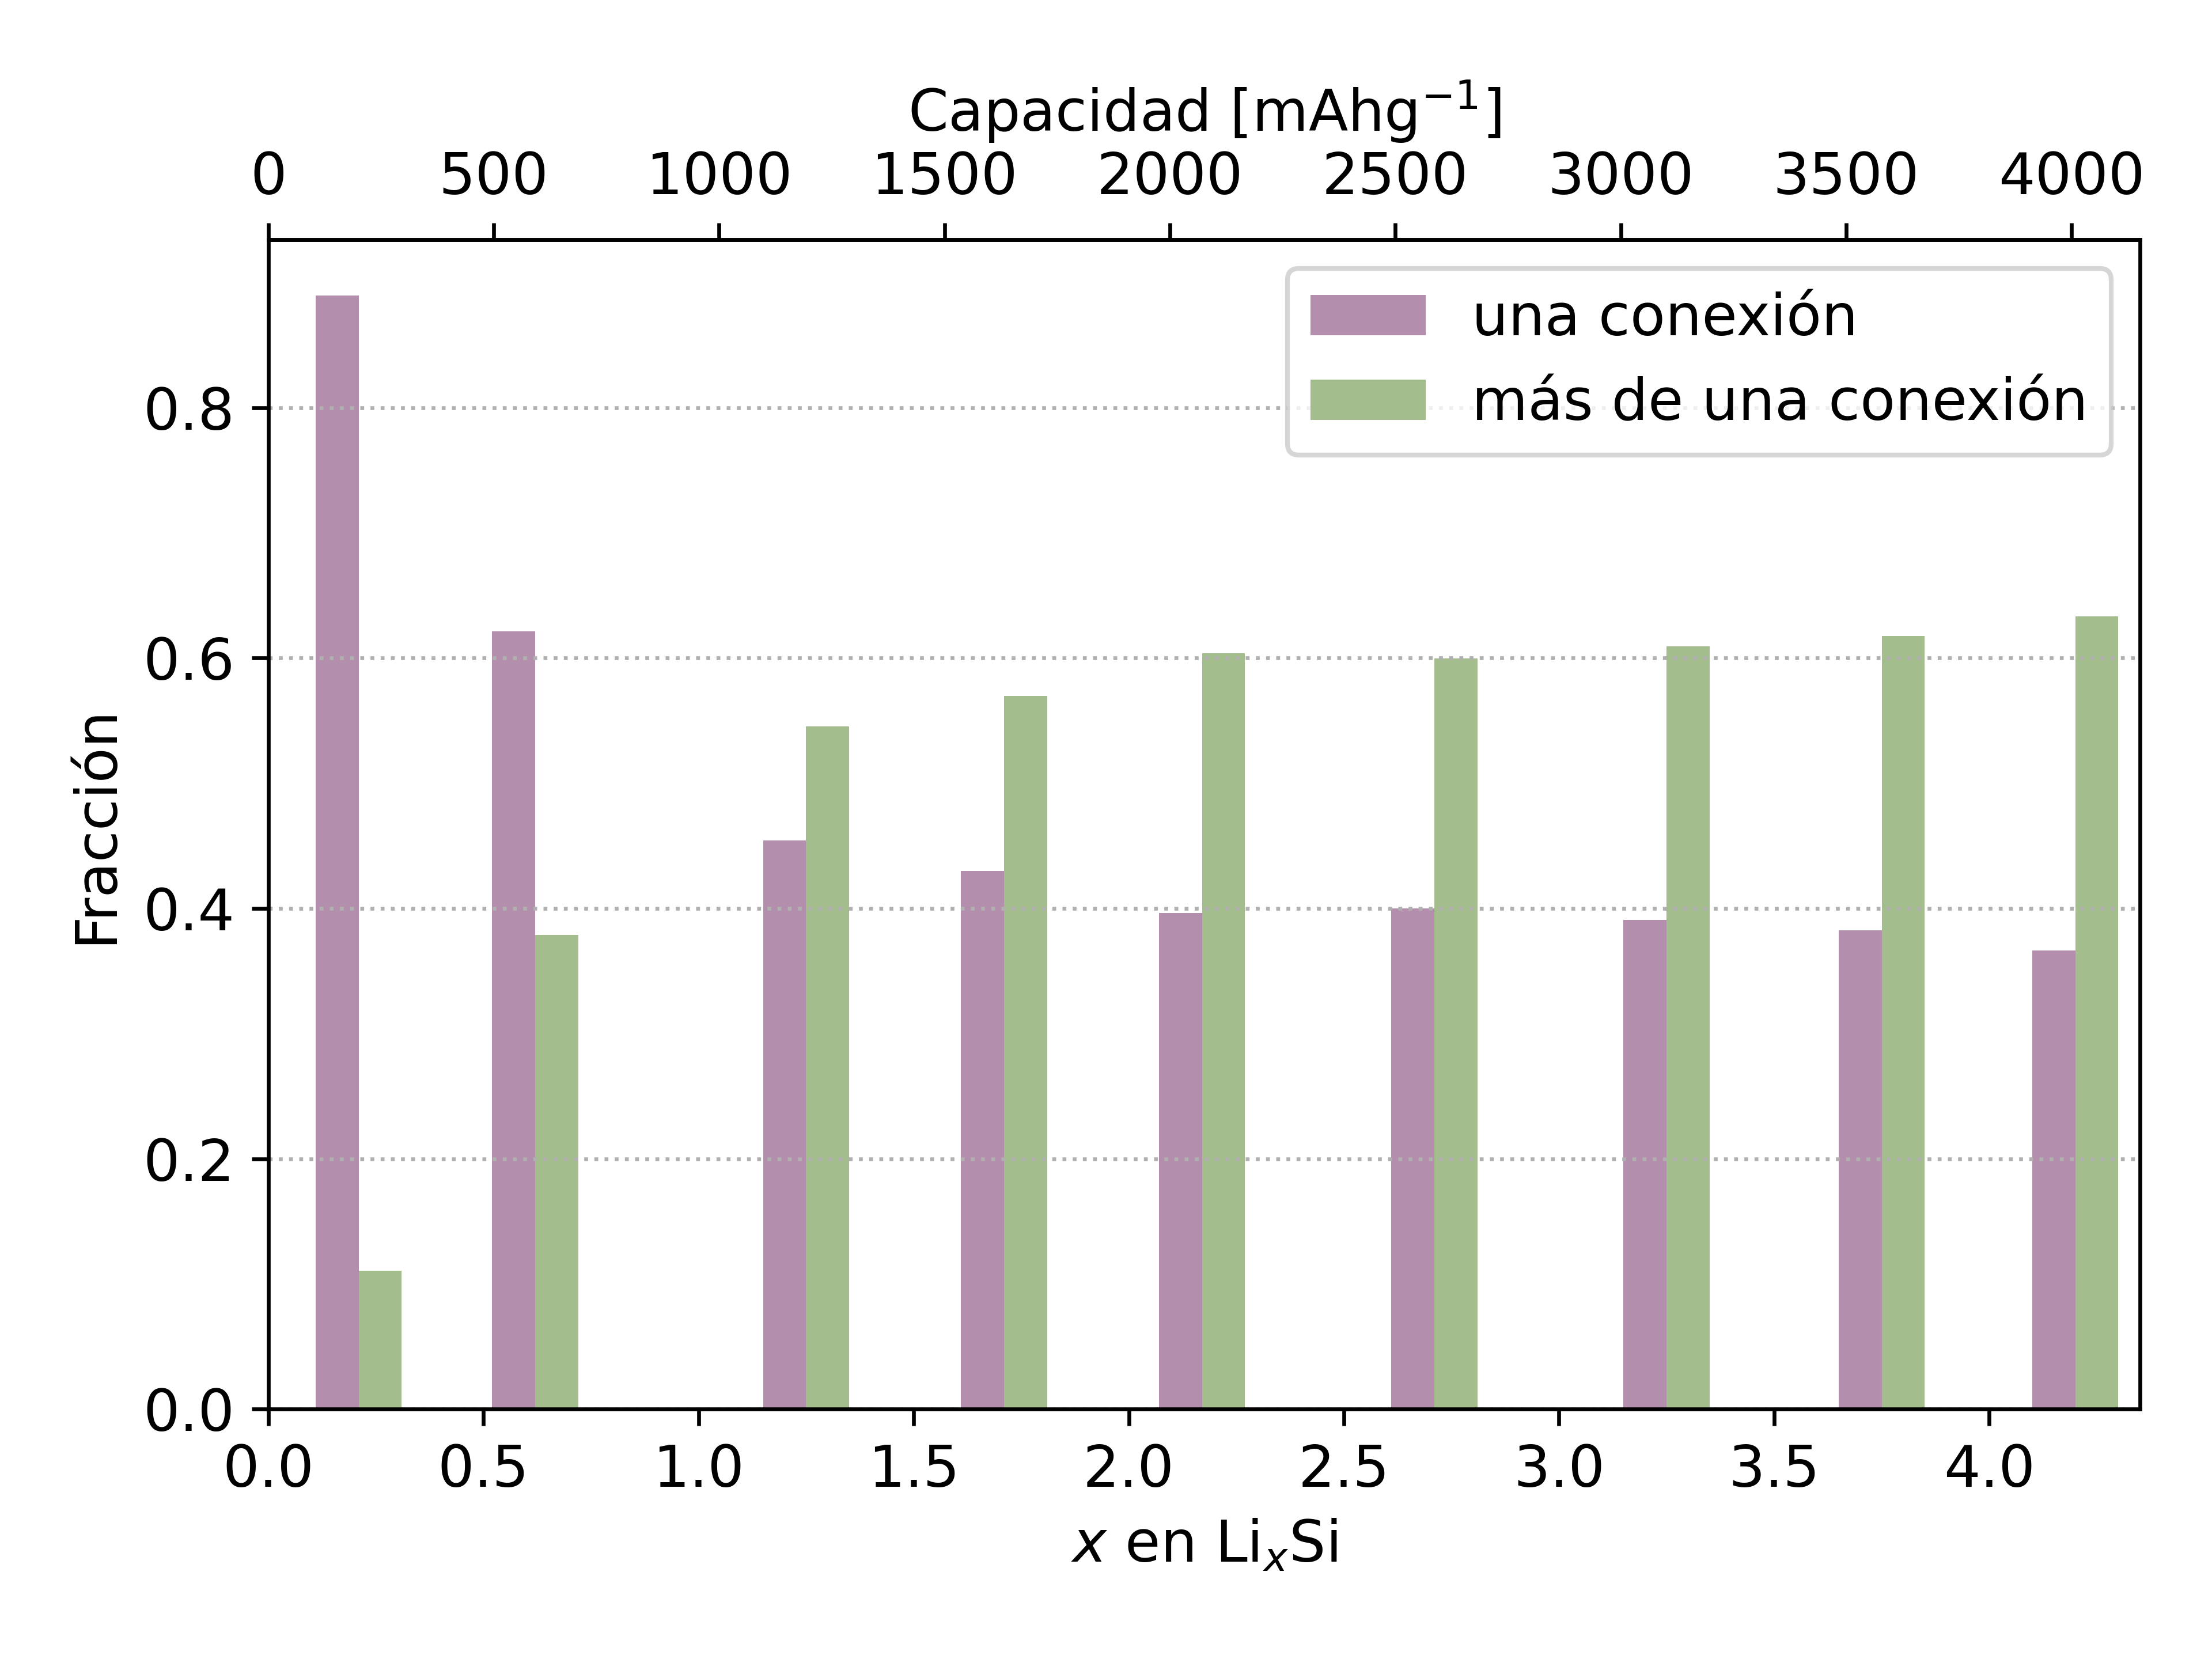
\includegraphics[width=0.7\textwidth]{Silicio/caracterizacion/resultados/interconexion/interconexiones-areas.png}
    \caption{Evolución con la concentración de la fracción que representa cada
    categoría de interconexiones de Li al área total del segundo pico de la 
    RDF$_{Si-Li}$.}
    \label{fig:interconexiones-areas}
\end{figure}


\subsection{Orden de corto alcance}

El término orden de corto alcance (SRO, de sus siglas en inglés 
\textit{short-range order}) se utiliza para denotar el ordenamiento de los átomos
que rodean a uno específico en una cáscara. Del mismo modo, el término 
\textit{clustering} se ha definido como la tendencia de los átomos similares a 
estar cerca unos de otros. Ambos conceptos se refieren a un orden estructural 
entre átomos vecinos, pero no son necesariamente persistentes a distancias más 
largas. Warren ~\cite{warren69} y Cowley ~\cite{cowley1950} definieron un 
parámetro (WCP) para caracterizar estos tipos de ordenamientos de la siguiente 
manera:
\begin{equation}
    WCP = 1 - \frac{p_{A-B}}{m_B} = 1 - \frac{p_{B-A}}{m_A},
\end{equation}
donde $p_{A-B}(p_{B-A})$ es la probabilidad de tener un átomo de tipo B(A) como
vecino de un átomo de tipo A(B) y $m_B(m_A)$ es la concentración global de átomos
B(A), expresadas en fracciones molares. La igualdad, en ambas definiciones 
posibles del WCP, viene del hecho de que la probabilidad de encontrar a un átomo 
de tipo A como vecino de un átomo de tipo B es igual a la de tener un átomo de 
tipo B como vecino de un átomo de tipo A, esto es $m_A p_{A-B} = m_B p_{B-A}$.

Los valores que se obtienen de utilizar el parámetro WCP en sistemas del tipo
A$_x$B indica una aleatoriedad completa si es igual a cero, preferencia por 
átomos de distinto tipo si $WCP < 0$ y preferencia por átomos del mismo tipo si 
$WCP > 0$. Aunque este parámetro permite un análisis cuantitativo notable, sólo
se define para sistemas cristalinos en los que cada átomo tiene el mismo número
de vecinos. ~\cite{warren69}

A continuación se extiende esta idea para definir un nuevo parámetro, 
$\theta_{A-B}$, que es adecuado para caracterizar estructuras amorfas, de la 
siguiente manera:
\begin{equation}
    \theta_{A-B} = \ln \left( \frac{C_{A-B}}{C_{Bulk}} \right),
\end{equation}
donde A indica la naturaleza del átomo que se considera como central y B el tipo
de átomo que se considera como vecino, equivalente a la definición de WCP. En
este caso, la relación entre la concentración local y la concentración global se 
calcula a partir de la integración de la distribución radial de a pares parcial,
$g_{A-B}(r)$, en una esfera al rededor del átomo central,
\begin{equation}
    \frac{C_{A-B}}{C_{Bulk}} = \frac{1}{V(r_{cut})} \int_0^{r_{cut}} g_{A-B}(r) dV,
\end{equation}
donde $r_{cut}$ y $V(r_{cut})$ son el radio de corte y el volumen de la esfera 
considerada. Ya que en $g_{A-B}(r)$ no hay dependencia angular, $dV$ puede 
escribirse como $4 \pi r^2 dr$. Esta cantidad puede pensarse como la 
concentración promedio dentro de la esfera relativa a la del material 
masivo. Así, de forma análoga al parámetro de WCP, $\theta_{A-B}$ indica 
la tendencia SRO o el \textit{clustering} para cualquier tipo de átomo dado.
Si $\theta$ es positivo, indica una acumulación de átomos relativa al 
\textit{bulk}, mientras que si es negativo indica una disminución. Si es igual a 
cero se tiene una aleatoriedad completa. Este nuevo parámetro también satisface 
la relación $\theta_{A-B} = \theta_{B-A}$ de la misma manera que se discutió para
el parámetro de WCP, ya que por definición $g_{A-B}(r) = g_{B-A}(r)$. Por lo cual 
se tiene que el parámetro $\theta_{A-B}$ da información similar a la que provee 
el WCP, pero además es aplicable a sistemas amorfos.

La figura \ref{fig:sro} muestra la variación del parámetro $\theta$ en función 
de la concentración de Li. Hay tres posibilidades para el análisis de $\theta$ en
sistemas de Li$_x$Si ($\theta_{Li-Li}$, $\theta_{Si-Si}$ y $\theta_{Si-Li}$), ya
que $\theta_{Si-Li} = \theta_{Li-Si}$. Para todos los casos se consideraron los
mismos radios de corte que en los cálculos del número de coordinación, luego del
primer pico de la RDF correspondiente.
\begin{figure}[th]
    \centering
    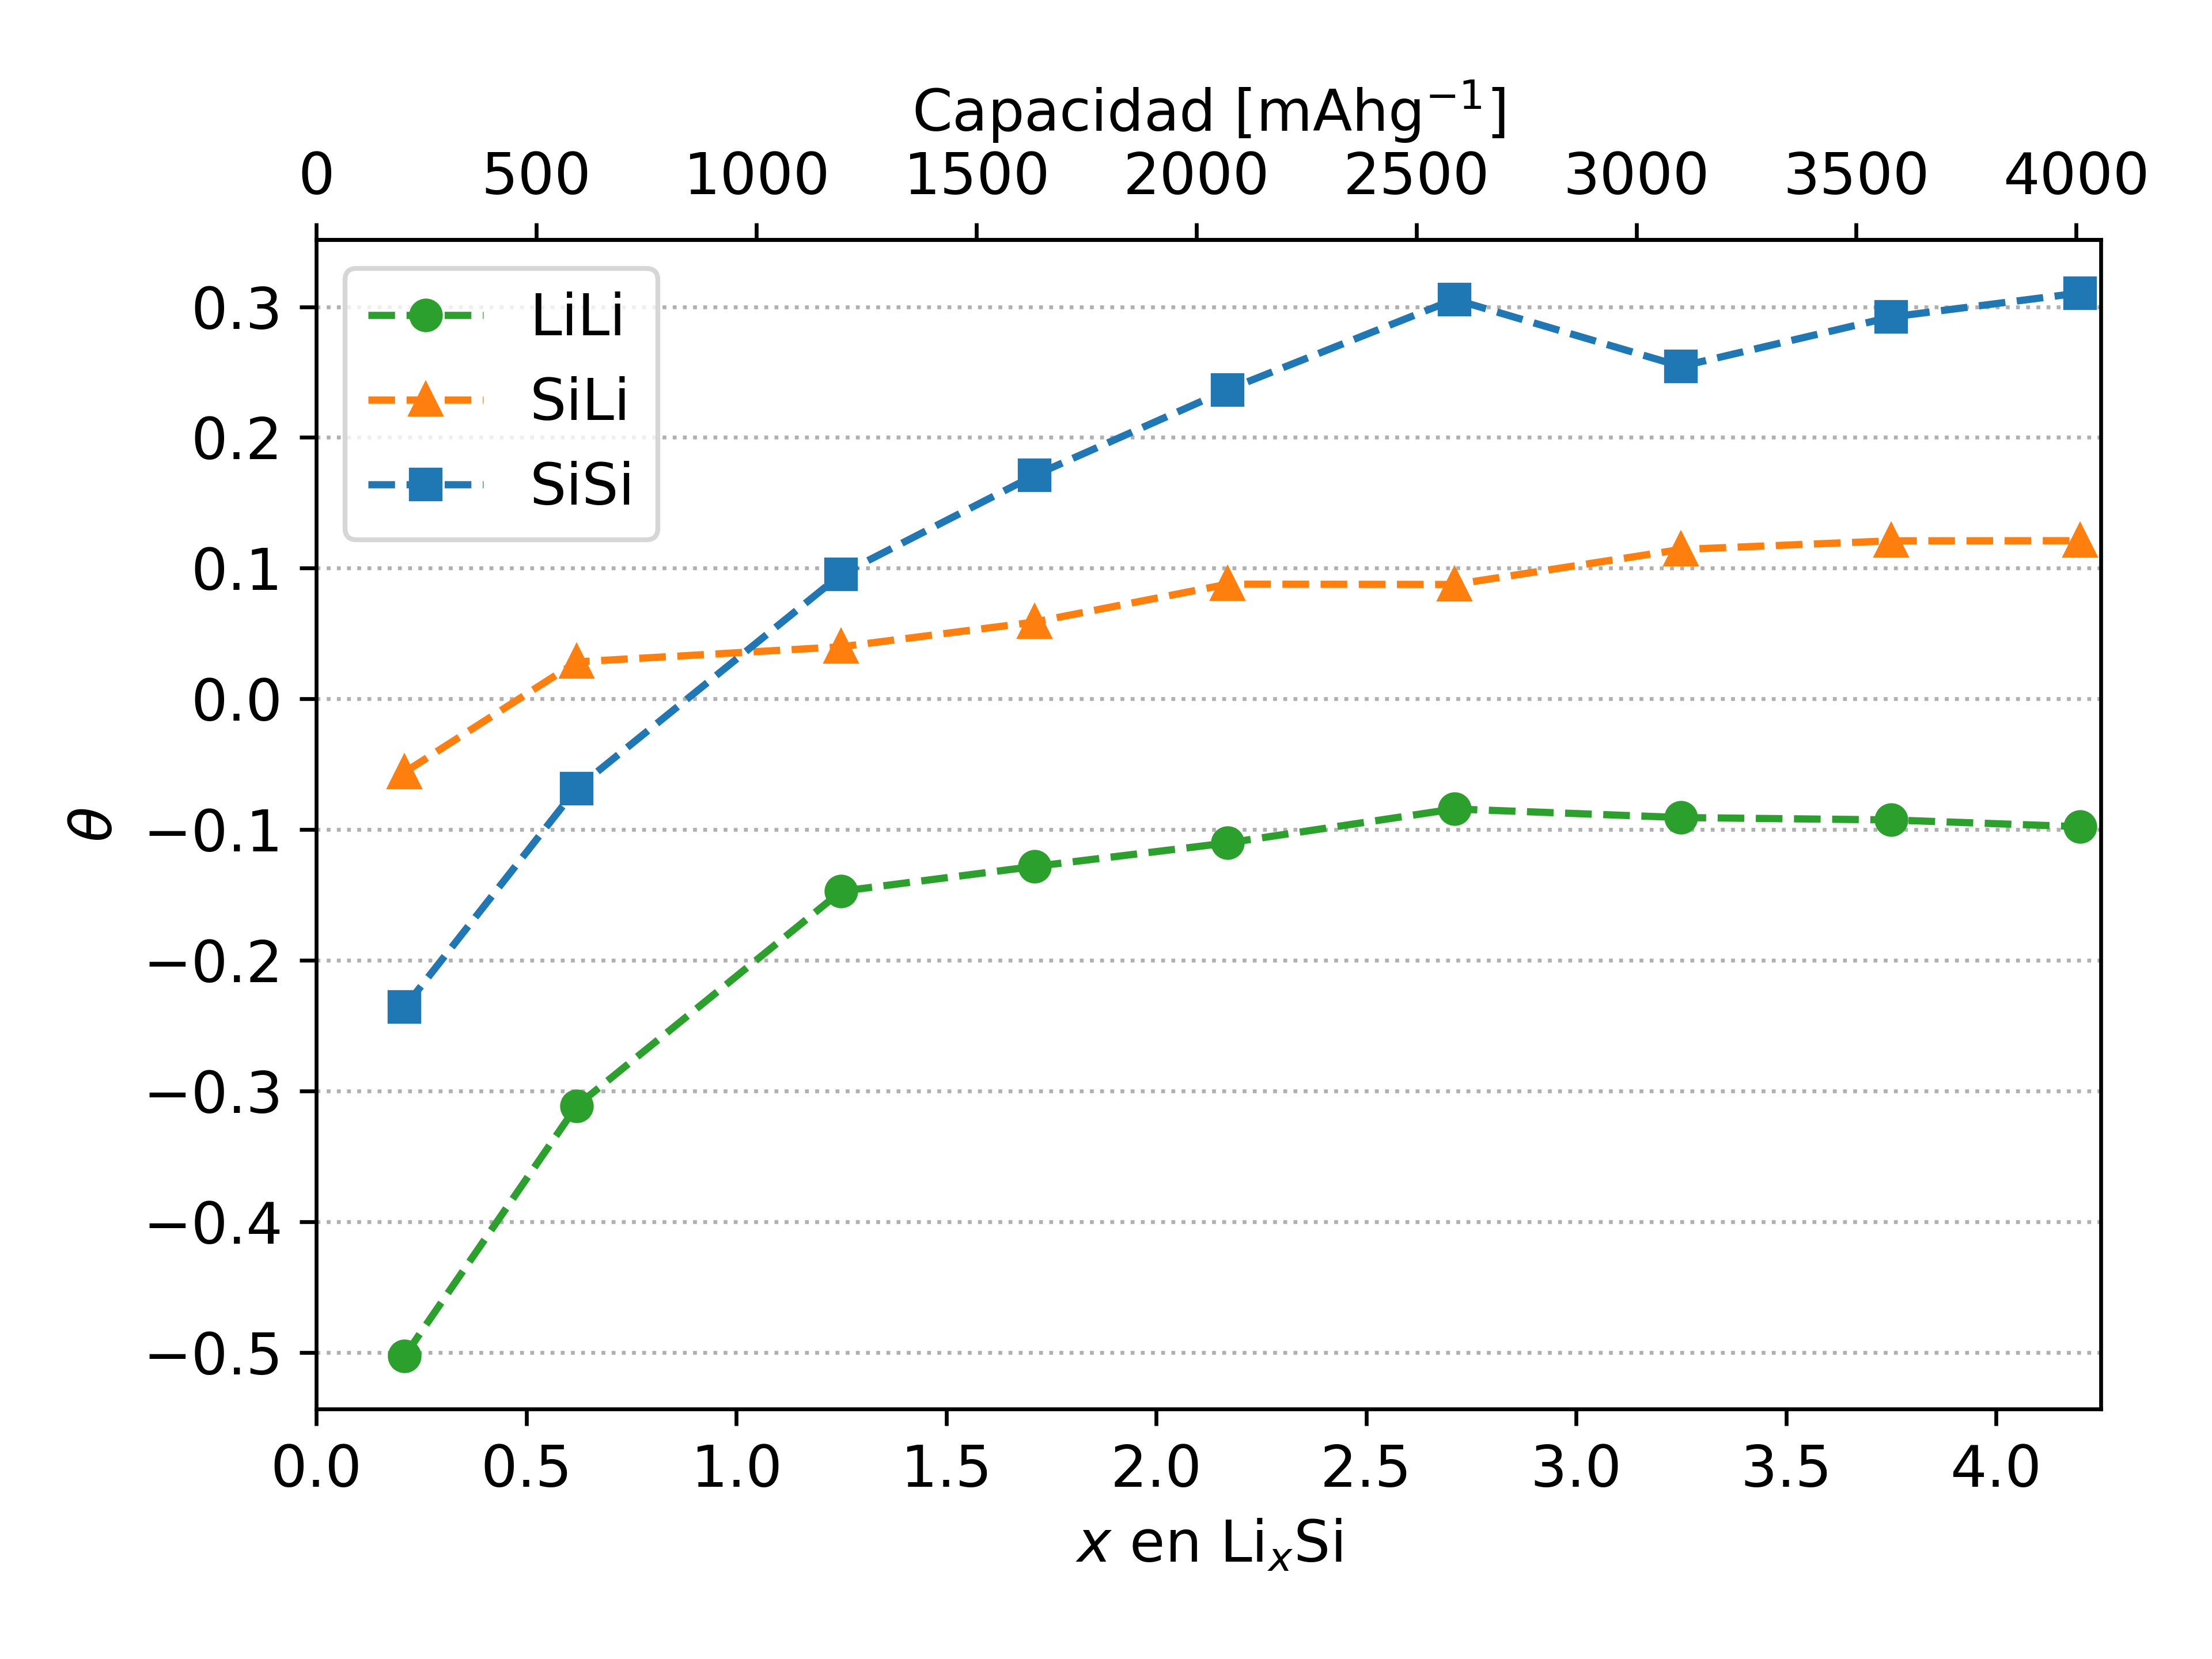
\includegraphics[width=0.8\textwidth]{Silicio/caracterizacion/resultados/sro/sro.png}
    \caption{Parámetros $\theta_{Li-Li}$, $\theta_{Si-Li}$ y $\theta_{Si-Si}$ 
    en función de la concentración de Li. El primer subíndice indica el tipo de
    átomo que se considera como central mientras que el segundo es el vecino. El
    radio de corte se eligió luego del primer pico de la RDF correspondiente.}
    \label{fig:sro}
\end{figure}

Como tendencia general, puede notarse que todos los valores de $\theta$ aumentan
cuando crece la cantidad de litio en el sistema, $x$, y que se estabiliza para 
valores grandes de $x$. Este comportamiento monótono y la disminución en la 
pendiente para concentraciones altas está correlacionado con el comportamiento
presentado en el análisis de los números de coordinación.

En el caso de $\theta_{Si-Si}$, alcanza un valor positivo aproximadamente 
constante para $x > 2.5$, mostrando una correlación fuerte con la presencia de 
cadenas lineales de Si, previamente discutidas y observadas en la figura 
\ref{fig:amorfas}. Aunque la presencia de estas cadenas se puede inferir a partir
de los valores de los CN en $x$ altos, $\theta$ es más sensible al SRO, ya que
está normalizado por la concentración global. Esta propiedad de $\theta$ permite
un análisis más claro incluso si las cadenas están interactuando entre sí, como
es el caso para concentraciones bajas de litio.

$\theta_{Si-Li}$ presenta variaciones pequeñas y un valor positivo para todo 
$x > 0.5$, mostrando una acumulación constante de Li al rededor del Si, o, 
análogamente, una acumulación de Si alrededor del Li. Este comportamiento se le 
puede atribuir a la interacción atractiva fuerte en los pares Si-Li. En el caso de 
$\theta_{Li-Li}$, este parámetro es siempre negativo, lo que indica una 
interacción débil Li-Li y la correspondiente disminución de vecinos Li-Li. Por
último, el parámetro $\theta_{Si-Si}$ tiene un valor negativo para $x < 1.0$, 
sugiriendo que la presencia de concentraciones bajas de litio tiende a separar 
los átomos de silicio entre sí. Sin embargo, $\theta_{Si-Si}$ se vuelve positivo
para $x > 1.0$, implicando una acumulación de vecinos de Si sobre átomos de Si, 
relativo a la concentración global. Esto se debe a la formación de estructuras 
Si-Si. Para $x > 2.5$ puede observarse un valor constante de 
$\theta_{Si-Si} \approx 0.3$, revelando la formación de estructuras estables de 
Si-Si dadas por las cadenas previamente mencionadas.



% Copyright (c) 2024, Francisco Fernandez
% License: CC BY-SA 4.0
%   https://github.com/fernandezfran/thesis/blob/main/LICENSE
\section{Conclusiones del capítulo}

Con el fin de emular las estructuras amorfas encontradas en muchos experimentos 
electroquímicos, en este capítulo se generaron por computadora estructuras desordenadas de 
aleaciones de Li$_x$Si para varios valores de $x$ utilizando un algoritmo de 
dinámica acelerada y un campo de fuerzas reactivo. La exploración acelerada de 
mínimos locales (AELM) permitió la caracterización de una amplia gama de 
estructuras amorfas. El cambio de volumen de las estructuras litiadas en relación 
con el Si está en concordancia con los resultados experimentales de microscopía de fuerza atómica. Las
energías de las estructuras obtenidas representan bien el comportamiento 
electroquímico de la curva de potencial en función de la concentración de Li. Se 
analizó la función de distribución radial de a pares para los diferentes tipos de 
pares atómicos y se dilucidó la estructura compleja del segundo pico del RDF 
Si-Li mediante un análisis de interconexión de clusters. Además, haciendo un 
análisis de la formación de clústeres en función del radio de corte, se demostró 
que las estructuras amorfas no presentan diferentes enlaces de Si ni átomos de Si 
aislados. En su lugar, se encontró que el sistema se comporta como una red amorfa.
Estudiando los números de coordinación de primeros y segundos vecinos para las 
diferentes concentraciones, se mostró que esta red amorfa mantiene las conexiones 
tetraédricas para bajas concentraciones de Li y que tiende a formar cadenas lineales para 
altas concentraciones de Li. Por último, la definición de un nuevo parámetro 
permitió determinar el orden de corto alcance de las estructuras amorfas, definido
por interacciones débiles Li-Li e interacciones fuertes Li-Si y Si-Si. El método propuesto AELM 
resulta ser un método rápido y eficaz para obtener mínimos energéticamente 
relevantes. Se hizo una analogía con el templado simulado múltiple.% Un análisis 
%detallado de la eficiencia de AELM en comparación con otros métodos eficientes 
%como el templado simulado múltiple o los métodos de Monte Carlo es una motivación 
%para trabajos futuros.

